\setcounter{chapter}{1}         % permet de débuter l'intro à 1. au lieu de 0.
\setcounter{section}{0}
\chapter*{Introduction}         % enlève la numérotation
\phantomsection\addcontentsline{toc}{chapter}{Introduction} % inclus l'intro dans la table des matières
\label{chapter:intro}

La plasticité du transcriptome face aux nombreuses perturbations qu'il subit permet à un organisme de préserver ses fonctions vitales en tous temps dans une certaine mesure. Par un appel à de nombreux mécanismes de régulation de l'expression des gènes, les cellules vont alors contrer, compenser ou limiter l'impact de la perturbation. Si les mécanismes majeurs de la régulation ont pu être identifiés dès les premières quantifications de l'expression, le récent développement des technologies de transcriptomique a permis d'accélérer cette tendance. La recherche en médecine moléculaire s'est donc emparée de cet outil dans une démarche d'identification systématique de la fonction de gènes encore mal connus ou de la cause de leur implication dans une maladie, un phénotype ou une condition.

La quantité de données faisant, le besoin de méthodes d'analyse biostatistiques capables de gérer autant d'information pour en ressortir des biomarqueurs significatifs s'est accru. C'est dans ce contexte qu'on a vu l’essor des méthodes d'analyse par réseau en biologie \cite{Barabasi2004} et plus particulièrement celles dites de réseau de co-expression de gènes. Par leur capacité à saisir l'ensemble des variations les plus subtiles dans le transcriptome et les variations conjointes entre gènes, les réseaux de co-expression de gènes ont su montrer leur intérêt dans la recherche de biomarqueurs de maladies complexes et encore irrésolues telles qu'Alzheimer \cite{Hu2020Nov} ou le cancer du sein \cite{Garcia-Cortes2020Jul}. Pourtant, leur emploi reste encore limité aux équipes possédant l'expertise d'un·e bio-informaticien·ne, retardant leur potentiel pour l'étude de nombreux phénomènes. Parmi eux, le vieillissement y gagnerait pourtant à utiliser des approches par réseau. De nature complexe, le vieillissement est un phénomène qu'on résume encore trop souvent à sa seule composante de sénescence. Il est pourtant le résultat de nombreux mécanismes entrecroisés que la co-expression est à même de décomposer grâce à son étude à l'échelle d'un système et pas seulement de ses acteurs individuels, les gènes.

Le but de mes travaux durant mon doctorat a donc été divisé en deux parties : i) tester la pertinence du développement d'un outil d'architecture pipeline modulaire, sous forme de paquet R, contenant une aide à l'interprétation et visant à pérenniser l'analyse de co-expression de gènes au vu de l'évolution des méthodes pour la réaliser, ii) évaluer le potentiel de découverte de l'analyse de co-expression de gènes à travers différents tissus pour une meilleure compréhension du vieillissement humain en priorisant des gènes. 

Cette introduction vise à donner les clefs essentielles à la compréhension des différents concepts biostatistiques, bio-informatiques et médicaux employés tout au long de cette thèse. Elle est suivie par deux chapitres dont le premier est la présentation de l'outil \textit{GWENA} dédié à l'analyse de réseaux de co-expression de gènes et de son application sur l'étude du vieillissement du muscle squelettique. Le second chapitre est une étude à plus large spectre du vieillissement analysant les fonctions communes à spécifiques du vieillissement à travers 10 tissus humains. S’ensuivent une conclusion résumant les apports de mes travaux, puis une discussion les replaçant dans le contexte des connaissances actuelles et les perspectives futures dans ce domaine.




\section{La complexité du vivant}

\subsection{Un fonctionnement multiple issu d'un code unique}

Le vivant est fait d'une diversité d'organismes à l'image de sa complexité. Chacun de ces organismes est composé d'une ou plusieurs cellules œuvrant ensemble pour la survie et la reproduction de celui-ci. Ces êtres multicellulaires sont bien souvent constitués d’une association de cellules à la fonction et la forme bien différentes de ses voisines. Ainsi, chez des organismes constitués d'un très faible nombre de cellules comme les Myxozoa constitués au maximum de 7 cellules \cite{Morris2010Aug} tout comme chez des organismes de taille bien plus importante comme l'humain fait d'entre 10\textsuperscript{12} et 10\textsuperscript{16} \cite{Bianconi2013}), on retrouve des cellules spécialisées pour une fonction spécifique \cite{Panina2020Sep} (Figure \ref{fig:intro_tissu_type_cellulaire}) \todo{à refaire en schematique ou à citer ou faire une figure avec la dernière table de cette page https://www.proteinatlas.org/humanproteome/celltype}. Celles-ci servent différents objectifs tels que la protection, l'acheminement d'éléments nutritifs, ou encore la transmission de matériel génétique. Chez l’humain, ces cellules seront par exemple respectivement des kératinocytes \cite{Yuki2007Apr}, des cellules endothéliales de l’intima \cite{Yuan1991Aug}, des ovocytes \cite{Trounson2013}. En s’assemblant entre cellules de même type, puis en formant des complexes avec d’autres types cellulaires, les organismes parviennent à former alors des structures nommées \textit{tissus} \cite{Hekselman2020Mar}. La combinaison de kératinocytes, de mélanocytes, de cellules de Langerhans et les cellules de Merkel connectées par une matrice extra-cellulaire forment ainsi le tissu épidermal, ou plus simplement l’épiderme \cite{Bettley1965}.

\begin{figure}[hb!]
    \centering
    % 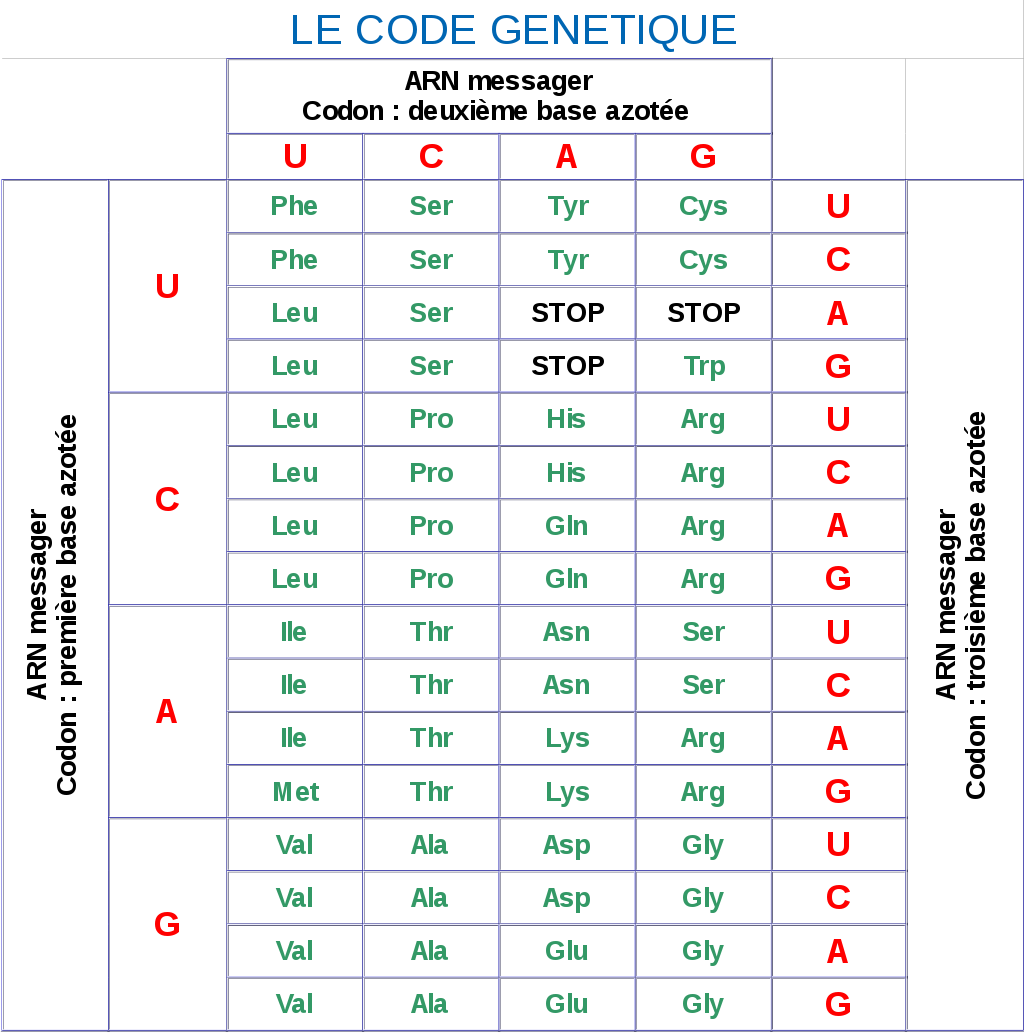
\includegraphics[width=0.95\textwidth]{img/intro/code_genetique.png}
    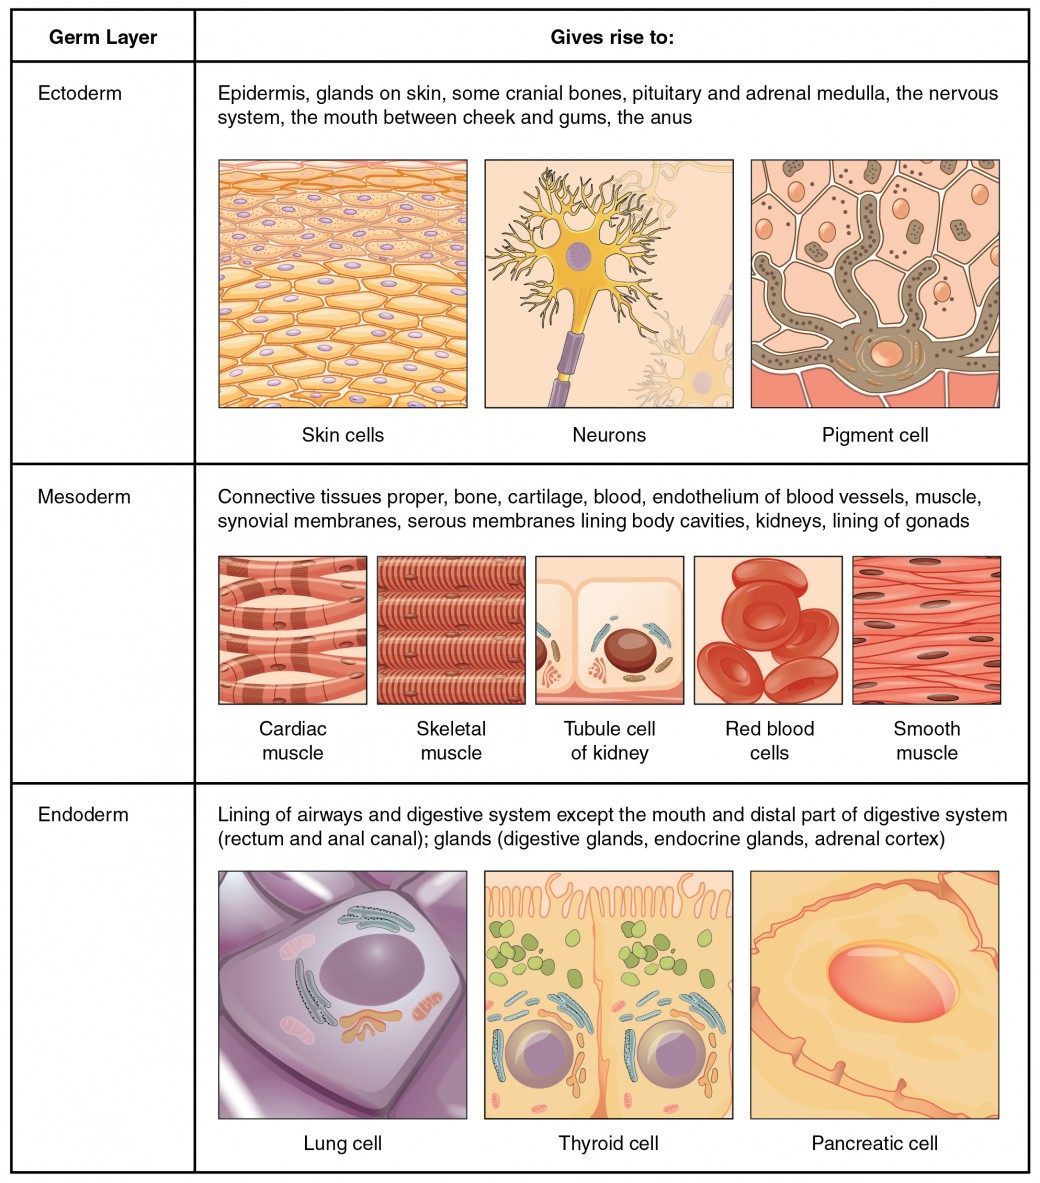
\includegraphics[width=0.8\textwidth]{img/intro/cell_type_feuillet.jpg}
    \caption{Exemple de la diversité de cellules selon le tissu et feuillet embryonnaire dont elles sont issues.}
    \label{fig:intro_tissu_type_cellulaire}
\end{figure}


Pour effectuer chacune de ces tâches spécialisées, les cellules de type différents vont produire en partie des protéines ayant des fonctions biologiques différentes de leurs voisines. Bien qu'il existe une très large diversité de fonctions, 32 catégories de fonctions selon le projet Gene Ontology \cite{Ashburner2000}, on peut toutefois les regrouper en 3 familles de fonctions majeures \cite{Mathews2012}:  
\begin{itemize}
    \item les fonctions catalytiques : les protéines, dans ce cas appelées enzymes, présentent une activité d'augmentation du taux de réaction chimique en diminuant l'énergie d'activation nécessaire. Ces enzymes sont spécifiques d'une transformation d'un substrat vers un produit. Elles peuvent cependant voir leur fonction altérée par des activateurs (co-facteurs, co-enzymes) et des inhibiteurs (co-répresseurs). Par exemple, la \textbeta-galactosidase va catalyser la transformation du lactose en glucose + galactose dans l'opéron lactose \cite{Jacob1961Jun}.
    \item les fonctions de signalisation ou liaison : en se fixant à un récepteur ou en étant un récepteur à la fixation d'un ligand, les protéines permettent de faire transiter de l'information en intra ou extra cellulaire. La fixation entraîne la transmission d'un signal physique ou chimique via une cascade d'événements qui vont conduire à une réponse cellulaire. Par exemple, la production d'une protéine d'insuline par le pancréas va, en se fixant sur les récepteurs membranaires des cellules, déclencher des mécanismes de stockage du glucose. Ce qui se traduit dans le foie par l'initiation de la transformation du glucose en glycogène.
    \item les fonctions de structuration : les protéines par leur forme et propriétés physico-chimiques hautement modulables permettent de donner une architecture ou des propriétés mécaniques aux cellules dans/autour desquelles elles se trouvent. Ex : la combinaison de protéines de myosine II et d'actine permettent la contraction musculaire par des phénomènes de coulissage de ces protéines.
\end{itemize}


Pour être produites, ces protéines suivent chacune un plan de construction défini dans le code génétique de la cellule. L'ADN~(Acide DesoxyRibinucléique) est le support de cette information génétique. L'ADN est un polymère de longueur variable selon les espèces et dont la séquence est composée de 4 types de nucléotides : adénosine, tyrosine, guanine et cytosine. Au long de sa séquence, l'ADN encode l'information relative aux protéines sous forme d'unité nommée \textit{gène}. Chez l'Homme (sur qui on se concentrera dans ce manuscrit) la version 37 de GENCODE [https://www.gencodegenes.org/human/stats.html] considère ainsi qu'il existe 60 651 gènes. Cependant, tous parmi eux ne produisent pas de protéine. On distingue en réalité les gènes dits "codants" (19951 toujours dans GENCODE 37) car produisant des protéines et les gènes "non-codants" qui codent pour plusieurs autres entités moléculaires utiles à la cellule.

Chez l'Homme et plus généralement les eucaryotes, l'ADN est contenu dans le noyau de la cellule où il se trouve condensé après plusieurs étapes de repliement à l'aide de protéines appelées histones. La machinerie cellulaire de production des protéines étant située à l'extérieur du noyau, une étape intermédiaire de transcription est nécessaire afin de copier la séquence ADN d'un gène sous la forme d'une molécule capable de sortir du noyau : l'ARN messager (ARNm). Semblable à l'ADN, l'ARNm est cependant mono brin alors que l'ADN est double brin. Dans ce système la thymine est remplacée par l'uranine. La taille d'un brin d'ARNm est plus petite que celle d'un fragment d'ADN car il n'embarque que l'information correspondant à un gène seulement. Chacun des triplets de nucléotides sur sa séquence (les codons) encode pour un des 20 types d'acides aminés constituant la protéine associée (Figure \ref{fig:intro_code_genetique}).

\begin{figure*}[!ht]
    \centering
    % 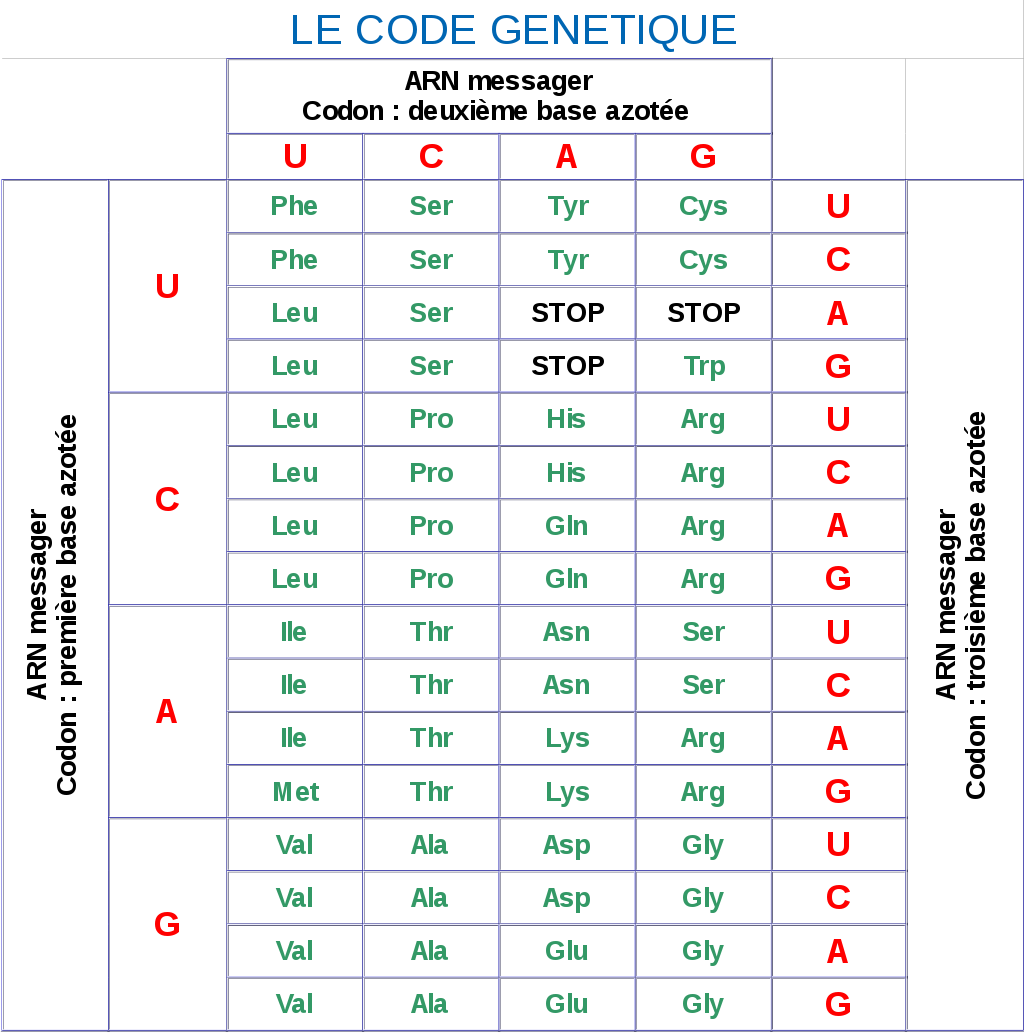
\includegraphics[width=0.95\textwidth]{img/intro/code_genetique.png}
    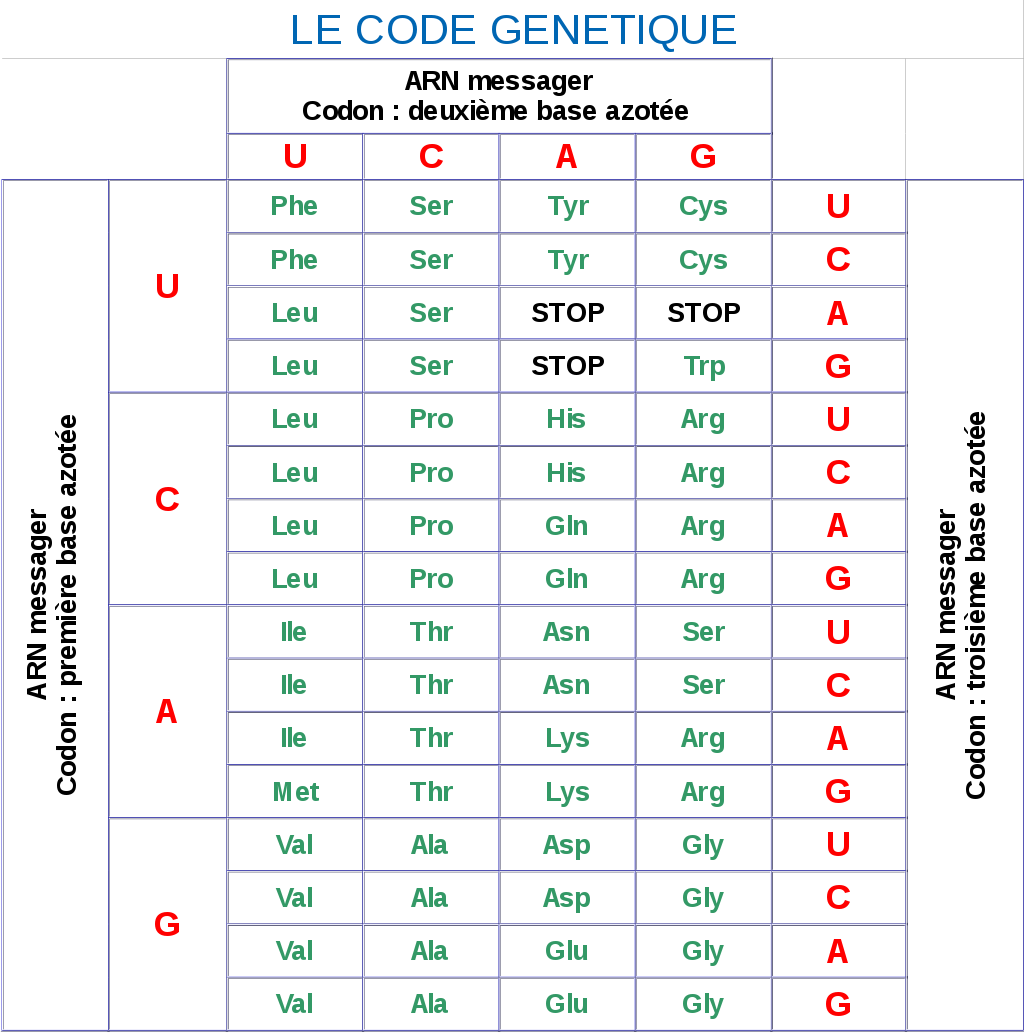
\includegraphics[width=0.8\textwidth]{img/intro/code_genetique.png}
    \caption{Correspondance de triplets de nucléotides avec l'acide aminé produit.}
    \label{fig:intro_code_genetique}
\end{figure*}


Une fois copié depuis l'ADN, l'ARNm immature, composé de sous unités appelées introns et exons, sort du noyau vers le cytoplasme pour subir une étape de maturation durant laquelle il se voit retirer ses introns et certains exons ou sections d'exons selon les besoins de sous-fonction de la protéine finale. On nomme "transcrits", les différentes version d'ARNm issues d'un même gène (Figure des modes d'épissage alternatif). Ainsi, on considère que la transcription d'un gène sous n'importe lequel de ses transcrits correspond à l'expression de son gène dans un échantillon. Par la suite, une étape de traduction de l'ARNm en polymère d'acides aminés donnera la base de la protéine. Après le repliement du polymère et des modifications dites "post-traductionnelles" par la machinerie cellulaire, la protéine sera enfin opérationnelle pour réaliser la fonction qui lui incombe. 


\subsection{La régulation de l'expression pour une spécification cellulaire}

Comme mentionné précédemment, l'ADN est identique dans toutes les cellules d'un organisme, alors même que chaque cellule n'est capable d'exprimer que les gènes spécifiques à sa fonction (de la myosine pour les myocytes, de la kératine pour les kératinocytes, etc.). Cette capacité des cellules est permise par les différents mécanismes de régulation de l'expression des gènes (et par extension leur répression) qui sont établis dès les premières différenciations cellulaires au cours du développement d'un organisme. Tous ces mécanismes, dits de régulation, sont interconnectés pour ajuster en temps réel la quantité de protéines nécessaires au fonctionnement immédiat de la cellule \cite{Weake2010Jun}. On distingue les mécanismes suivants : 
\begin{itemize}
    \item \textbf{La régulation de l'initiation de la transcription} : lors de la transcription de l'ADN d'un gène en ARNm, l'accessibilité des régions cis-régulatrices dépend de l'impact de plusieurs éléments de régulations parmi lesquels on retrouve les amplificateurs (\textit{enhancers} en anglais) et les inactivateurs (\textit{silencers} en anglais), des séquences riches en motifs de liaison de facteurs de transcription capables respectivement d'augmenter ou diminuer le niveau d'expression des gènes \cite{Levo2014Jul}. Très souvent présents dans des boucles de rétro-action, ces facteurs de transcription qui sont des protéines peuvent eux-mêmes voir leur expression augmentée ou diminuée par des acteurs variés tels que des ARN non-codants et des protéines \cite{Chen2020May}.
    % ZaZo0o : l'expression spatiotemporelles des gènes est conférée par l'action conjointes de l'accécibilité des résions cis-régulatrices et de la présences de facteurs de transcription. Parmis les séquences régulatrices, on retrouve les séquences enhancers, qui sont des séquences riches en motifs  de facteurs de transcription, et sont capable d'activer et de booster le niveau d'expression des gènes de mannière tissus-spécifique.
    % lors de la transcription de l'ADN d'un gène en ARNm, l'ARN polymérase chargée de la transcription vient se fixer sur l'ADN sur le site d'initiation de la transcription (appelé promoteur) pour ensuite commencer à lire la séquence. La fixation au préalable d'une protéine sur ce site (facteur de transcription) entraine alors l'impossibilité de fixation de l'ARN polymérase chargée de la transcription ou à l'inverse favorise son recrutement pour la transcription du gène visé. Très souvent présents dans des boucles de rétro-action, ces facteurs de transcription peuvent ainsi être eux-mêmes inactivés par des substances variées. L'exemple le plus connu est l'opéron lactose : en présence de lactose dans la cellule, le facteur de transcription (répresseur) lacl est inactivé par la fixation de lactose sur lui-même et de la \textbeta-galactosidase codée par le gène lacZ est produite. En l'absence de lactose, il est libre de se fixer sur le promoteur lac qui est le site d'initiation de la transcription pour les gènes lacZ, lacY, et lacA.
    \item \textbf{La conformation de la chromatine} : les repliements de l'ADN pour la condenser dans une cellule implique de rendre spatialement disponibles certaines régions à la transcription et indisponibles d'autres \cite{Kadauke2009Jan}. La variation d'accessibilité dans ces régions est notamment due du niveau de compaction des boucles que forme la chromatine avec elle-même.
    \item \textbf{La modification post-transcriptionnelle} : les ARNm nécessitent l'ajout d'une 7-methylguanosine sur l'extrémité 5' (coiffe 5'), un épissage et une polyadénylation sur l'extrémité 3' (l'ajout d'une queue poly A) afin d'être traduits en protéine. En l'absence de ces modifications, les ARNm sont détruits par la cellule \cite{Mercer2010Nov}.
    \item \textbf{La méthylation} : les îlots CpG situés sur l'ADN (notamment dans les promoteurs) peuvent subir l'ajout d'un groupement méthyl, empêchant alors la fixation de différents agents de la transcription \cite{Gutierrez-Arcelus2013Jun}.
    \item \textbf{La susceptibilité à la dégradation} : afin de perdurer plus de quelques minutes dans la cellule, certains ARN contiennent ou évitent des motifs de nucléotides influant la vitesse de dégradation (éléments riches en AU, codon stop prématuré, taille de queue poly-A) \cite{Yu2001}. Des ARN non-codants tels que les ARN interférants de petite taille (ARNip), les ARN micro (ARNmi) et les ARN longs non codants (ARNlnc) peuvent également favoriser la dégradation de certains ARN cibles \cite{Patil2014Jan}.
    \item \textbf{La régulation de la traduction} : en perturbant l'initiation, l'élongation ou la terminaison de la traduction des ARNm, des acteurs tels que les fragments dérivés d'ARN de transfert (ARNt) \cite{Krishna2021Mar}, le niveau de ribosomes disponibles \cite{Khajuria2018Mar} ou encore des ARNmi \cite{Meijer2013Apr}.
\end{itemize}


\todo{Figure mixée de celle de ZaZo0o et celle trouvée}



% 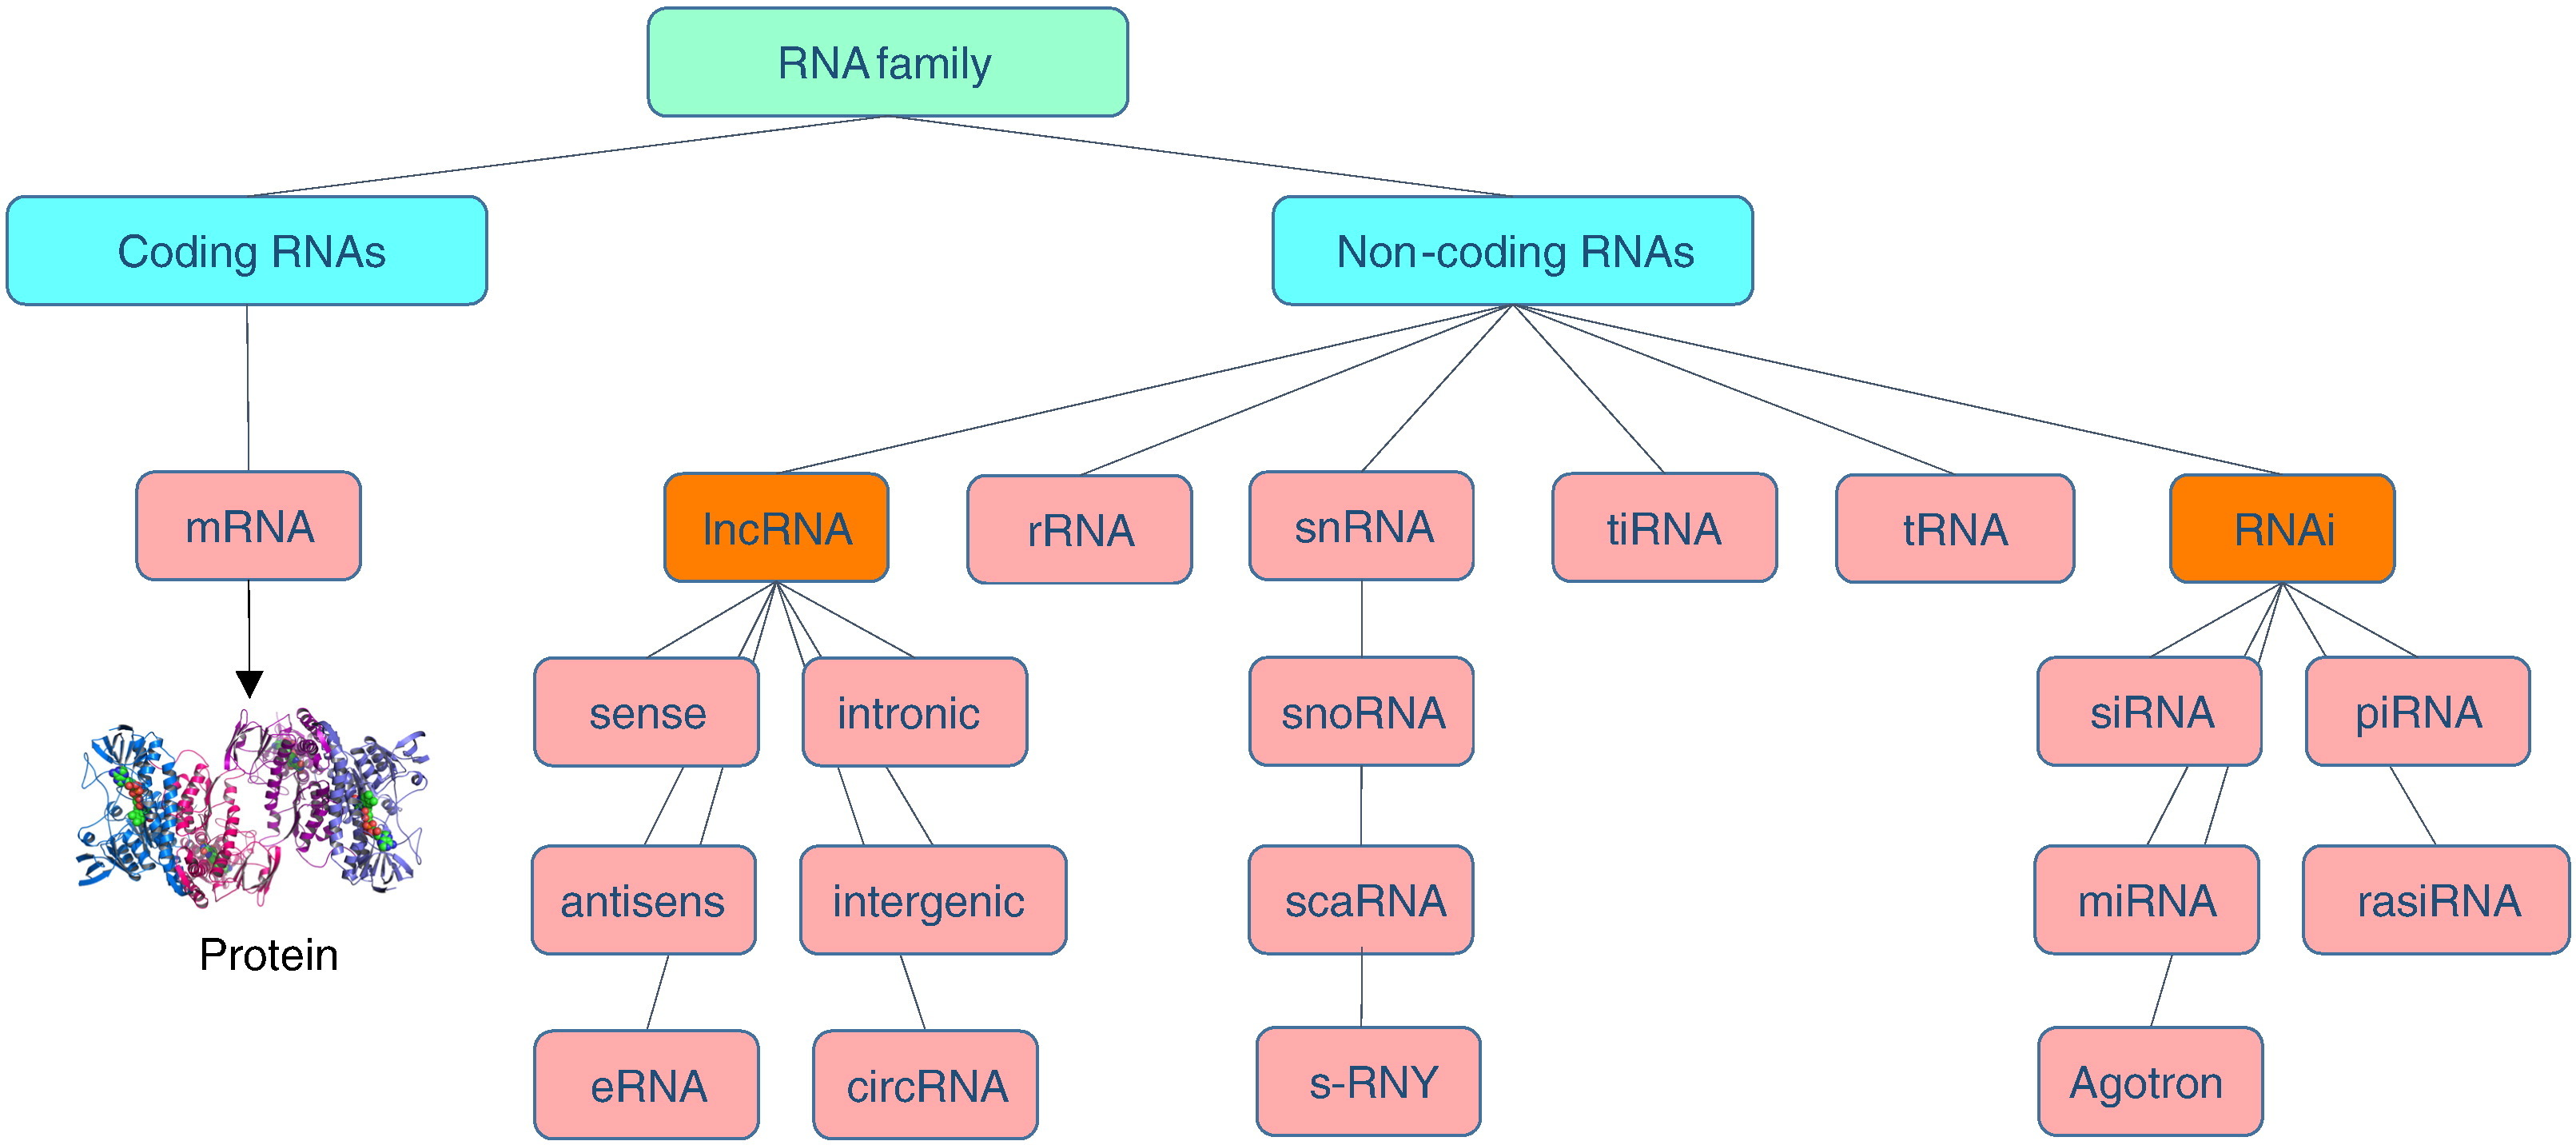
\includegraphics{img/intro/rna_familly_tree.jpg} %% https://www.sciencedirect.com/science/article/pii/S0167488916302919

%% TRANSITION : parler des erreurs/variabilité biologique ? 

% \subsection{L'étude des perturbation du vivant pour la résolution de conditions cliniques}
\subsection{L'étude l'expression des gènes pour la résolution de conditions cliniques}


Qu'il s'agisse du génome entier, du génome de tissus ou du génome de cellule spécifiques, les études de profilage transcriptomique ont permis de mieux comprendre le fonctionnement basal et sain de ces entités \cite{Hughes2000, Cloonan2008Jul}. Aussi appelées "approches systématiques", ces études servent en premier lieu à identifier de gènes impliqués dans des fonctions physiologiques (annotation) \cite{Munji2019Nov}, à associer des régions de l'ADN à des traits quantitatifs (locus de caractère quantitatif LCQ ou \textit{QLT} en anglais) \cite{Sarkar2019Apr}, ou encore à identifier des mécanismes de régulation de la transcription \cite{Segales2016Dec} ou des mécanismes cellulaires tels que la différenciation \cite{Godoy2018Jul}, la réparation de l'ADN \cite{Jividen2018Dec}, etc. De plus en plus de ces études permettent par la suite une réutilisation de ces données en les déposant dans des répertoires en ligne tels que Gene Expression Omnibus (GEO) \cite{Barrett2013Jan} et ArrayExpress \cite{Athar2019Jan}. Ils ont notamment été utilisées pour créer Expression Atlas \cite{Lukk2010Apr}, une carte globale d'expression des gènes avec une mise à jour récente pour inclure des données provenant du séquençage de cellules uniques \cite{Papatheodorou2020Jan}. Ces données ainsi que la connaissance associée par les études dont elles sont issues permettent alors d'avoir une vision générale du fonctionnement sain de l'humain pour mieux étudier par contraste les perturbations qui occurrent.

% Lors des perturbations du fonctionnement cellulaire par une maladie, le stress, l'âge, la régulation de l'expression se retrouve altérée. Le transcriptome, ensemble des ARN ou transcrits produits, est alors un témoin direct des fonctions mises en défaut \cite{Morozova2009Aug}. L'étude de la quantité de chaque transcrit exprimé donne alors un moyen direct de comprendre l'origine de manifestations macroscopiques (irritation atopique, tumeur, nécrose, etc.) ou moléculaires (augmentation du taux de glucose, malabsorption de nutriments, augmentation du pH, etc.) observables.
Ces perturbations du fonctionnement cellulaire peuvent provenir de différentes conditions telles qu'une maladie, une mutation, un stress, ou encore l'âge. Avec chacune d'elle, la régulation de l'expression se retrouve altérée différemment par rapport au fonctionnement sain. Le transcriptome, ensemble des ARN ou transcrits produits, est alors un témoin direct des fonctions mises en défaut \cite{Morozova2009Aug}. 

L'étude de la quantité de chaque transcrit exprimé donne ainsi un moyen direct de comprendre l'origine de manifestations macroscopique tel que la présence de tumeur ou nécrose dans les tissus. Ce type d'étude permet également une compréhension plus fine des variations moléculaires telles que des variations de pH ou la mauvaise absorption de nutriment dans l'organisme. En recherchant les transcrits dont la quantité change significativement entre une personne saine et une personne affectée par la condition considérée, il est alors possible d'isoler des biomarqueurs de la condition en question. Outre leur rôle d'aide au dépistage de certaines conditions, les biomarqueurs ont un intérêt en termes de soin car ils peuvent représenter ce qu'on nomme une cible thérapeutique. En conceptualisant des molécules en fonction du biomarqueur, on peut être capable d'interférer avec le biomarqueur, ses précurseurs, ses co-acteurs ou ses produits, le tout en vue de limiter leurs potentiels impacts négatifs.

%% Suite de paragraphe ?
% Un point sur la différence d'expression d'un point de vue global ou d'un point de vue tissu spécifique ?

%% Transition
La détection fiable de ces biomarqueurs est alors primordiale et dépend tant de la méthode de quantification des transcrits que de leur analyse.

%% Sources d'aide à la rédaction
% https://www.mdpi.com/1422-0067/18/8/1652/htm#B4-ijms-18-01652 : Transcriptome Profiling in Human Diseases: New Advances and Perspectives
% Intro utile pour retravailler cette section : https://www.nature.com/articles/nrg.2017.96

%% Infos potentiellement rajoutables :
% - On s'est intéressés tardivement au transcriptome historiquement car on pensait que tout le non codant était du "junk DNA". Ça a changé avec l'arrivée en 2000 du premier génome humain (https://www.ncbi.nlm.nih.gov/pubmed/5065367/). Formulation "De la première version du génome humain dans les années 2000 à sa dernière version complète en 2021, l'analyse du génome humain a permis de désavouer l'hypothèse du junk DNA. On ne considérant plus le génome non-codant comme inutile, l'étude du transcriptome au complet a permis de nombreuses perspectives d'études sur des conditions cliniques alors dans une impasse.

\section{Les technologies de transcriptomique pour la quantification de l'expression des gènes}

% Depuis leur démocratisation dans les années 80, les techniques de séquençage ont largement évolué au point qu'on distingue à présent 3 générations. La première génération, bien que plus d'actualité, a permis la première tentative de séquençage du transcriptome humain \cite{}. % <- c'est dans le cadre du sequencage genomique qu'on parle de générations
\subsection{Historique des technologies de transcriptomique}

L'ARN est une molécule dont la stabilité est faible et la dégradation rapide en raison des nombreuses enzymes de dégradation la ciblant dans une cellule. Les premières technologies de transcriptomiques utilisent donc rarement les ARN en eux même et vont plutôt construire des ADN complémentaires (ADNc) de leurs séquences à l'aide de transcriptases reverse découvertes en 1970 \cite{Temin1970Jun}. Ces premières technologies de transcriptomique furent basées sur les marqueurs de séquence exprimée (MSE ou en anglais \textit{expressed sequenced tags}), de courtes séquences d'ADNc identifiantes de transcrits qu'on détectait ensuite par migration sur gel. Développés au début des années 70, les MSE ont servi de base à la méthode SAGE (\textit{Serial Analysis of Gene Expression}) créée en 1995 \cite{Velculescu1995Oct} qui analyse les MSE concaténés via le séquençage Sanger lui-même inventé en 1975 \cite{Sanger1975May} et technique de séquençage alors très populaire à l'époque \cite{Marra1998Jan}. Cette méthode, dite rétrospectivement de "bas débit", a permis les premiers séquençages de transcriptome partiel \cite{Jeppesen1970Apr} ou complet pour des organismes à ARN de petite taille \cite{Fiers1976Apr}. La quantification par réaction en chaine d'ARN retro transposé (RT-qPCR de l'anglais \textit{reverse transcription quantitative polymerase chain reaction}) combinée à un buvardage de northern (en anglais \textit{northernblot}) fut également utilisée à partir de la fin des années 80 en raison de sa grande précision sur la quantification de transcrits \cite{Becker-Andre1989Nov}.
% Les premières technologies de transcriptomique furent basées sur les marqueurs de séquence exprimée (MSE ou en anglais \textit{expressed sequenced tags}), de courtes séquences de cDNA identifiantes de transcrits. Développés au début des années 70, les MSE ont servi de base à la méthode Sanger inventée en 1975 \cite{Sanger1975May} qui deviendra une technique de séquençage très populaire \cite{Marra1998Jan}. Cette méthode, dite rétrospectivement de "bas débit", a permis tant le séquençage des ARN que leur quantification. Les premiers séquençages de transcriptome partiel \cite{Jeppesen1970Apr} ou complet pour des organismes à ARN de petite taille \cite{Fiers1976Apr} ont ainsi été réalisés à l'aide de ces méthodes via MSE. La quantification par réaction en chaine d'ARN retro transposé (RT-qPCR de l'anglais \textit{reverse transcription quantitative polymerase chain reaction}) combinée à un buvardage de northern (en anglais \textit{northernblot}) fut également utilisée à partir de la fin des années 80 en raison de sa grande précision sur la quantification \cite{Becker-Andre1989Nov}.


\begin{figure}[!ht]
    \centering
    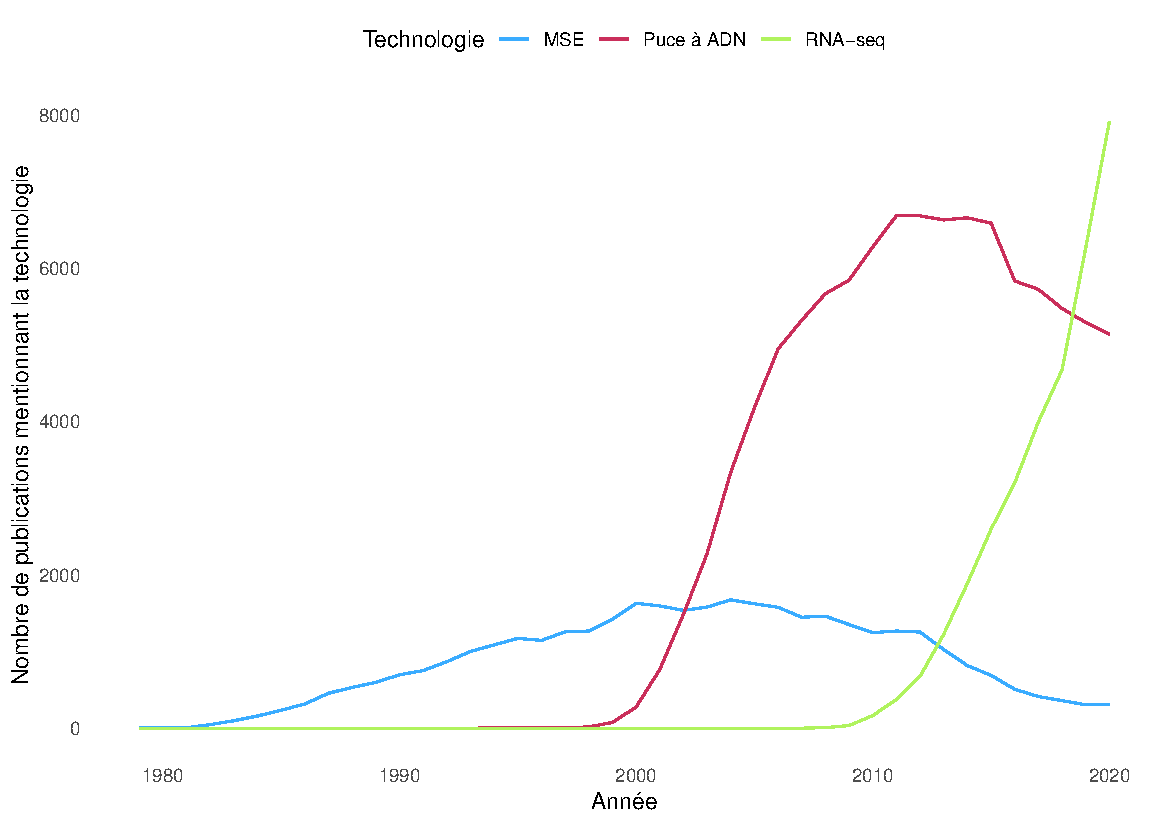
\includegraphics[width=\textwidth]{img/intro/count_by_year_rnaseq_microarray_est.pdf}
    \caption[Évolution de l'utilisation des différentes techniques de transcriptomique en se basant sur le nombre de publications les mentionnant]{Évolution de l'utilisation des différentes techniques de transcriptomique en se basant sur le nombre de publications les mentionnant. Les résultats proviennent du site PubMed (\url{https://pubmed.ncbi.nlm.nih.gov}) avec les requêtes suivantes : \textbf{MSE} = "cDNA library" OR "cDNA libraries" OR "complementary DNA library" OR "complementary DNA libraries" OR "expressed sequence tag" OR "expressed sequence tags", \textbf{Puce à ADN} = "micro array" OR "microarray" NOT "chromosomal", \textbf{RNA-seq} = "RNA Seq" OR "RNA-Seq" OR "RNASeq".}
    \label{fig:count_by_year_rnaseq_microarray_est}
\end{figure}


L'utilisation de SAGE et de RT-qPCR dans l'étude de l'expression des gènes a toutefois diminué dans les années qui ont suivi au profit de nouvelles technologies capables de quantifier un plus grand nombre de transcrits simultanément \cite{Lowe2017May}. Les puces à ADN par hybridation (en anglais \textit{hybridation-based microarrays}) ont ainsi été prisés dès le milieu des années 90 \cite{Schena1995Oct} après la commercialisation de la première puce Affimetrix \cite{Lenoir2006} en raison de leur faible rapport coût sur transcrits quantifiés. Cependant, face à la contrainte des puces à ADN de devoir connaître les séquences des transcrits à quantifier, la technologie du RNA-seq est devenue un incontournable dans nombre d'études. 
Profitant de l'amélioration des technologies de séquençage génomique via toujours une rétro-transposition de l'ARNm en ADNc, la technologie du RNA-seq va émerger dans les années 2000 et est annoncée comme révolutionnaire \cite{Wang2009Jan}. Toutefois, sa mention dans une publication n'arrivera qu'en 2008 \cite{Nagalakshmi2008Jun} bien que la technologie ait été utilisée pour des données publiées dès 2006 \cite{Cheung2006Dec}.

Les puces à ADN et le RNA-seq sont encore aujourd'hui les deux technologies de quantification de l'expression des gènes utilisées, malgré le déclin annoncé des puces à ADN (Figure \ref{fig:count_by_year_rnaseq_microarray_est}). Les bio-informaticien·ne·s sont donc amené·e·s à devoir traiter et analyser les données issues de chacune en tenant compte des propriétés biologiques, techniques et statistiques respectives à chacune des deux technologies.


%% Sources d'aide à la rédaction
% Un TRES bon site sur les technos de sequencage : http://education.knoweng.org/sequenceng/

%% Infos potentiellement rajoutables :
% - L'importance et l'impact du projet de séquençage du génome humain sur les technologies de séquençage avec les retombée bénéfique pour la transcriptomique :  invalidation de l'idée de "junk DNA" et profit des techno dev pour la génomique grace a juste l'utilisation de cDNA pour transformer le RNA
% - La variété des techno transcripto qui s'est développée avec le scRNA-Seq, real time RNA-seq, etc.
% - Parler des l'impact de toutes ces technos sur le transcriptome humain ? Plutot dans une sections à part

\subsection{Les puces à ADN}

% \subsubsection{But et protocole}
\subsubsection{Principe}


Les puces à ADN modernes consistent en une lame de verre sur laquelle est déposé un ensemble de fragments d'ADN nommés amorces (en anglais \textit{probes}) dans des puits qui correspondent aux ARN que l'on souhaite quantifier. Les constructeurs de puces à ADN tels que Affymetrix, Illumina ou Agilent mettent donc à disposition plusieurs modèles d'amorces prédéfinies sur puce pour réaliser la quantification de l'expression de gènes chez un organisme \cite{Liu2010}. Certains laboratoires universitaires disposent également de l'équipement pour réaliser leurs propres puces avec des amorces sélectionnées pour une étude \cite{Thompson2001Apr}. Cette option est particulièrement pertinente lors de la quantification d'organismes à l'annotation récente, d'organismes non disponibles en puce chez les constructeurs ou bien lors d'étude sur des sous ensembles de transcrits par rapport aux librairies des puces constructeur.


Pour venir réagir avec les amorces de la puce, les transcrits sont tout d'abord isolés de l'échantillon par purification. Une étape de transcription inverse donne ensuite l'ensemble des cDNA capables d'être liés avec les amorces. Afin de quantifier par fluorescence l'hybridation des cDNA aux amorces, les cDNA sont associés à des marqueurs fluorescents. Certaines puces sont prévues pour une utilisation avec un seul marqueur et sont dites à un seul canal, tandis que d'autres sont à deux canaux et permettent alors l'hybridation de deux échantillons différents tels que deux conditions (ex : sain/malade, sauvage/muté, etc.) \cite{Bumgarner2013Jan}. Chacun est reconnaissable sur la puce car marqué avec des fluorochromes différents : la Cyanine 3 qui émet à  570 nm (vert) et la Cyanine 5 qui émet à 670 nm (rouge). Les puits contenant plusieurs amorces visant un même gène, une hybridation compétitive a lieu et permet pour un même transcrit de quantifier relativement chacun des échantillons \cite{Koltai2008Apr}. Après une étape de rinçage, les puces sont scannées par un laser qui va exciter les marqueurs fluorescent. Un détecteur équipé d'un capteur de fluorescence va mesurer l'intensité émanant de chaque puits et chaque longueur d'onde s'il s'agit d'une puce à deux canaux. Il en résulte une image, ou deux si il y a deux canaux, tel que visible en Figure \ref{}.LETTRE \todo[inline]{a preciser}.


\todo{Reprendre la figure en commentaire en rajoutant au début l'aspect extraction/purification} 
% https://www.researchgate.net/figure/DNA-Microarray-Hybridization-using-a-two-channel-and-b-single-channel-microarray_fig6_44227364



En parallèle de cette méthode la plus courante, d'autres méthodes existent pour la construction des puces à ADN. On a présenté ici la version par dépôt d'amorces, mais il existe aussi une méthode par synthèse \textit{in situ}. Cette méthode permet notamment l'utilisation d'amorces de plus grande taille (> 70 mers ou nucléotides) qui augmentent la spécificité \cite{Liu2010}. Certaines puces à ADN utilisent également des billes de polystyrènes à la place de la lame de verre pour la fixation des amorces et se servent de ratios entre deux colorations n'interférant pas avec la fluorescence pour identifier l'amorce \cite{Nesterov-Mueller2014Oct}. 

Afin de transformer les images obtenues, quelle que soit la technique, en une donnée exploitable, le signal détecté sur chacun doit ensuite être traité en fonction de la puce utilisée. Les puces à ADN sur lame de verre étant les plus courantes, on s'attardera par la suite sur leur traitement en particulier.

% Le signal détecté doit ensuite être traité en fonction de la puce utilisée 

% Principe de la puce à ADN/ARN
% Coloration mono/duo
% Préparation de librairie
% Construction des puces
% Exemples d'utilisation ?

% %% Infos potentiellement rajoutables :
% - Les autres utilisations posibles du microarray : https://en.wikipedia.org/wiki/DNA_microarray#Uses_and_types

% \subsubsection{Propriétés mathématiques/techniques et normalisation}
% \label{subsubsection:microarray_props_and_normalisation}
\subsubsection{Pré-traitement des données}

% En raison de la nature de capture du signal des puces à ADN, les données capturées sont de type continu. Il est donc possible de con

% La fluorescence des transcrits hybridés étant captée sous la forme d'un signal continu à intensité variable, les données issues de puce à ADN seront de même nature. Cette valeur qu'on nomme parfois "abondance" est par ailleurs relative car l'intensité du signal reçu est systématiquement rapportée sur le signal reçu sur un contrôle blanc, sans fluorescence (en anglais \textit{background}).

\begin{figure}[!h]
    \centering
    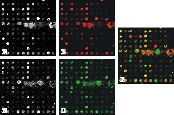
\includegraphics{img/intro/true_microarray_picture_10.1016_j.fss.2004.10.012.png}
    \caption[Image d'une puce à ADN à deux canaux rouge et vert]{Image d'une puce à ADN à deux canaux rouge et vert. (a) Canal rouge en échelle de gris, (b) Canal vert en échelle de gris, (c,d) Cannaux respectifs colorés selon leur fluorescence, (e) Puce à ADN visualisée en coloration RGB (\textit{Red Green Blue}). Des artefacts de fluorescence sont visibles en ligne 5. Issu de Lukac et al. 2005 \cite{Lukac2005May}.}
    \label{fig:true_microarray_picture_10.1016_j.fss.2004.10.012}
\end{figure}

L'intensité de fluorescence, aussi appelée abondance, détectée par le capteur constitue la donnée retournée pour un transcrit donné sur une puce à ADN en théorie. Comme on peut le voir en Figure \ref{fig:true_microarray_picture_10.1016_j.fss.2004.10.012}, cette abondance n'est toutefois pas uniforme au sein d'un même puits. L'image capturée va donc rarement être utilisée en tant que telle pour donner les abondances chiffrées finales et va passer par un premier ensemble d'ajustement.

En 2004, Petrov et al. \cite{Petrov2004Nov} ont ainsi exploré en détail l'impact de différents paramètres expérimentaux et de différents choix de correction du signal en se basant sur un contrôle qualité approfondit des puces étudiées. Le pré-traitement de l'image prise d'une puce à ADN y est découpé selon 4 étapes, plus une s'il s'agît d'une puce à deux canaux : l'alignement d'image (si deux canaux), le placement de grille, la détection de puits, la segmentation et la mesure de qualité (Figure \ref{fig:microarray_image_preprocessing}). Ces étapes permettent en finalité s'assurer une reproductibilité dans la valeur d'abondance détectée, ainsi qu'une robustesse face à des évènements tels que des artefacts de fluorescences, des contaminations de puits, ou encore des variations de fluorescence entre réplicats.

\begin{figure}[!h]
    \centering
    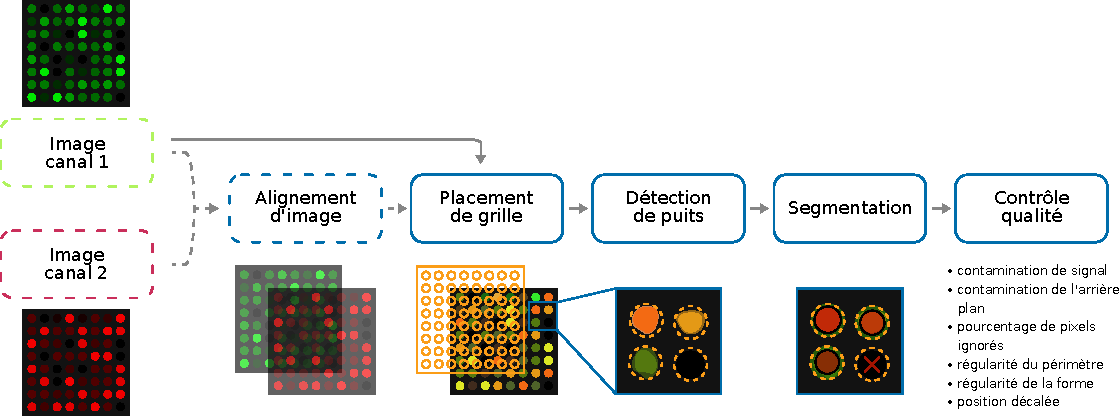
\includegraphics[width=\textwidth]{img/intro/microarray_image_preprocessing.pdf}
    \caption{Ordre des différentes étapes de pré-traitement d'une image de puce à ADN. Modifié d'après Petrov et al \cite{Petrov2004Nov}.}
    \label{fig:microarray_image_preprocessing}
\end{figure}

Une fois cette étape de traitement de l'image effectuée, de nombreux biais techniques peuvent encore impacter la valeur chiffrée retournée depuis l'image corrigée. On applique donc une étape dite de normalisation qui visera tant à palier les biais techniques contrôlables qu'incontrôlables afin de comparer au mieux différentes conditions. La variété de modèles de puces à ADN et de conditions d'utilisation peut demander l'utilisation de normalisations spécifiques, mais on retrouve communément 3 d'entre elles qui font consensus \cite{Smyth2003Dec} (Figure \ref{fig:microarray_normalization}) : la normalisation d'arrière-plan, la normalisation intra-puce, et la normalisation inter-puces.

% Si des normalisations consensus existent, la variété de modèles de puces à ADN et de conditions d'utilisation peut demander l'utilisation de normalisations supplémentaires. On se concentrera ici sur les normalisations consensus uniquement \cite{Smyth2003Dec} (Figure \ref{fig:microarray_normalization}) bien qu'on mentionnera brièvement d'autres normalisations plus contextuelles. 

La normalisation de l'arrière-plan va venir corriger le biais d'intensité parasite lié au phénomène d'hybridation non spécifique des transcrits sur les amorces dans les puits. Par une simple soustraction de l'intensité de l'arrière-plan à l'intensité détectée dans chaque puits on va permettre de compenser le biais. Lors de l'utilisation d'une puce à deux canaux, les intensités en fonction de la fluorescence utilisée tendent à ne pas couvrir le même intervalle d'intensité. Il est possible également que d'autres biais non-linéaires impactent les différents canaux de la puce. Ces biais sont corrigés par une normalisation dite intra-puce et n'est donc généralement pas utilisée dans le cas de puce à un canal. Plusieurs méthodes se sont succédé pour réaliser cette normalisation avec dans les débuts une utilisation d'un puits de contrôle, de la somme de toutes les intensités, ou de la déviation absolue médiane pour diviser les intensités de chaque transcrit. Plus récemment, l'approximation des données par une régression pondérée locale (en anglais \textit{LOESS} pour \textit{LOcally Estimated Scatterplot Smoothing}) inspirée du théorème de Taylor et aboutie par Cleveland et Devlin en 1988 \cite{Cleveland1988Sep} a prouvé être particulièrement efficace pour retirer ce biais intra-puce \cite{Smyth2003Dec}. Enfin, la finalité des puces à ADN dans l'analyse d'expression de gène étant la comparaison de conditions, on va effectuer une étape de normalisation inter-puces pour s'assurer de leur comparabilité pour détecter au mieux les variations significatives entre elles. Cette correction consiste donc à rendre similaire la distribution des intensités. La méthode variera cependant selon le type et le nombre de canaux des puces bien la plupart soient une adaptation d'une normalisation par quantiles \cite{Ritchie2015Apr}. \\

\begin{figure}[!h]
    \centering
    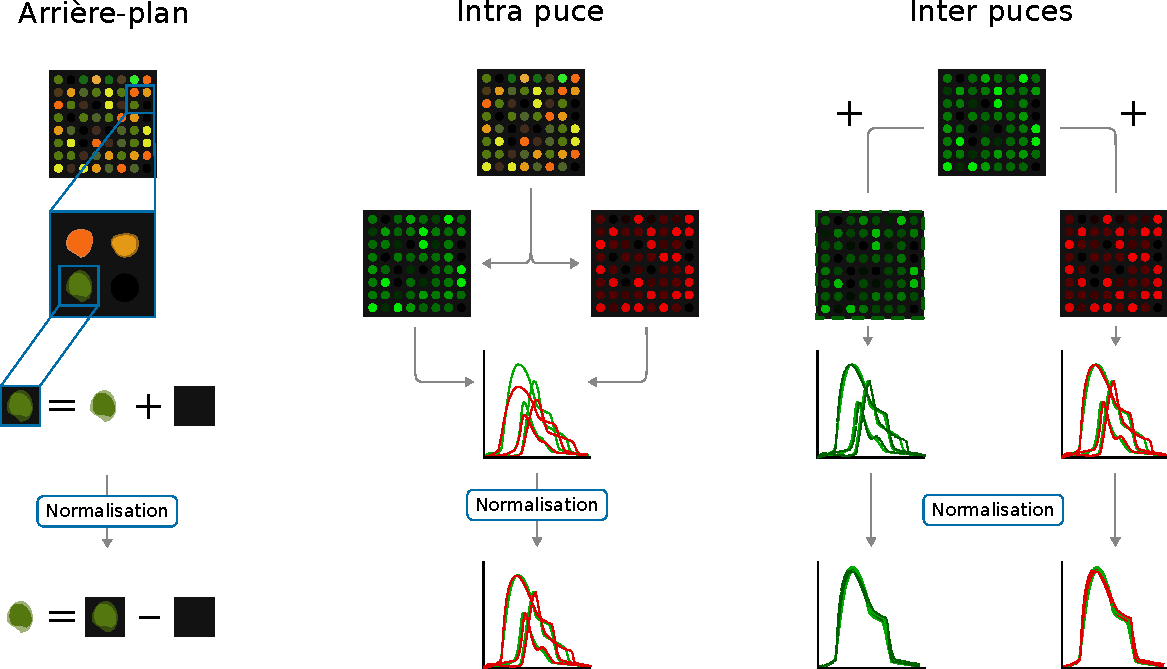
\includegraphics[width=\textwidth]{img/intro/microarray_normalization.pdf}
    \caption[Normalisations consensus de puces à ADN]{Normalisations consensus de puces à ADN : la normalisation de l'arrière-plan, la normalisation intra puce, et la normalisation inter puces.}
    \label{fig:microarray_normalization}
\end{figure}


À ces normalisation s'ajoutent d'autres transformations usuelles des données des puces à ADN telles que des filtrations \cite{Quackenbush2002Dec}. On y retrouve la suppression des données d'intensité des transcrits dont la fluorescence du puits aurait saturé le capteur et engendré une quantification tronquée \cite{Wilkes2007Apr}. Lors de l'utilisation de réplicats biologiques, les transcrits présentant une faible intensité après normalisation de l'arrière-plan et une faible variation entre les réplicats peuvent être supprimées des données. Également, il est d'usage de transformer les données d'intensité en log, le plus souvent un log2. Ce changement d'une expression en échelle additive en une échelle proportionnelle de facteur 2 vise à faciliter l'interprétation. En effet, dans cette disposition, une intensité augmentant ou diminuant de 1 unité signifiera respectivement un doublement ou une division par deux de l'intensité \cite{Smyth2003Dec}, ce qui est souvent considéré comme un changement de l'expression significatif en biologie. 

Ces différentes normalisations et transformations peuvent mathématiquement se réaliser dans n'importe quel ordre. Toutefois, bio-informatiquement, il est important de s'attacher à l'ordre et au choix des méthodes employées car chacune possède des contraintes, un contexte d'utilisation, et doit tenir compte du type d'analyse réalisée sur les données par la suite. On parle alors de stratégie de normalisation. Parmi les précautions à prendre dans la stratégie, il est par exemple nécessaire lors d'analyses comparatives de conditions de tenir compte des transcrits supprimés d'une des deux puces à ADN uniquement. Dans le cas contraire, une différence significative artificielle pourrait être obtenue, faussant alors les résultats. De même, l'étape de normalisation intra-puce doit être faite avec parcimonie car elle peut entraîner dans certains cas une non-comparabilité ultérieure avec d'autres puces en fixant la distribution relativement à la puce considérée \cite{Argyropoulos2006Apr}. Enfin, plus généralement, une utilisation à mauvais escient de certaines normalisations peut aussi entraîner une suppression du signal biologique d'intérêt. Une fois totalement préparées, ces données peuvent finalement être analysées par diverses méthodes pour détecter des différences biologiques.

% Le package R \textit{limma} hébergé sur le dépôt Bioconductor \cite{Gentleman2004Sep} regroupe l'intégralité de ces normalisations de même que d'autres outils de contrôle qualité et est ainsi devenu une référence dans la normalisation post traitement d'image et plus généralement l'analyse de puces à ADN.


Mais face à la limitation en nombre de transcrits et à l'impossibilité de quantifier des transcrits inconnus, l'utilisation de puces à ADN tend à diminuer de plus en plus au profit du RNA-seq. Bolon-Canedo et al. soulignent ainsi en 2019 \cite{Bolon-Canedo2019} qu'elles ne sont plus pertinentes à ce jour pour de la recherche exploratoire telle que l'étude du transcriptome de nouveaux organismes ou l'analyse comparative de l'expression dans des conditions mal comprises.
L'utilisation des puces à ADN reste toutefois pertinente dans d'autres types d'analyses plus ciblées de transcrits. Elles restent un outil au rapport qualité/prix imbattable dans des analyses de génotypage pour du diagnostic ou de l'étude de population.


%% Sources d'aide à la rédaction
% Un TRES bon site sur les technos de sequencage : http://education.knoweng.org/sequenceng/

%% Infos potentiellement rajoutables :
% RAjouter une explication d'en quoi consiste chaque étape ?

%% INFOS ET FORMULATION SUR LA NORMALISATION
% Parmi les biais biologiques classiques, on retrouve le contenu en GC, la longueur des transcrits, la quantité d'ARN total,  weighted linear regression (lowess).
% Pour corriger ces biais biologiques, plusieurs méthodes ont été proposées prenant chacune plus ou moins de biais en compte  : 
% linear regression analysis1, log cen- tering, rank invariant methods2 and Chen’s ratio statistics3
% SOURCE : 10.1038/ng1032


\subsection{RNA-Seq}

\subsubsection{Principe}

Aujourd'hui, le séquençage de l'ARN (RNA-seq) est devenu la technologie privilégiée pour les études transcriptomiques. Issue des techniques de séquençage nouvelle génération, le RNA-seq permet d'étudier le transcriptome d'un organisme sans connaissance préalable de sa séquence \cite{Wang2009Jan}. Le protocole de préparation des transcrits est le même que pour les puces à ADN sauf dans le cas d'un séquençage direct de l'ARN. Après prélèvement des échantillons, les transcrits sont isolés par purification et rétro-transcrits en ADNc. Ceux-ci sont alors amplifiés par PCR et fragmentés selon la taille requise par la technologie de séquençage. Le séquençage peut se faire actuellement par seconde ou troisième génération dépendant de l'objectif poursuivit. Les technologies de seconde génération, avec notamment celle d'Illumina (Figure \ref{fig:rnaseq_workflow}), sont ainsi adaptées dans le cadre d'une comparaison de conditions. Elles produisent rapidement un séquençage au rapport qualité prix raisonnable avec un minimum de 30 millions de lectures alignées recommandées par le projet ENCODE \cite{ENCODE2012} pour de l'ARN total chez l'homme. Les technologies de troisième génération telles que PacBio ou Nanopore (Figure \ref{fig:rnaseq_workflow}) sont quant à elles plus longues mais peuvent séquencer des fragments de taille bien supérieure à ceux de seconde génération. Cette capacité les rend donc particulièrement adaptée à l'analyse de la variété de transcrits issus de l'épissage alternatif \cite{Bergsma2018Jan}. Les lectures de ces fragments (en anglais \textit{read}) sont ensuite alignées sur un transcriptome de référence ou sont l'objet d'un assemblage de transcriptome\textit{de novo}. Plusieurs méthodes partant de différents postulats existent pour réaliser cette étape d'alignement loin d'être triviale. Chacune possède ses avantages et limites qu'il faut toutefois prendre en compte en cela qu'elles impactent l'expression finale quantifiée \cite{Yi2018Oct,Srivastava2020Dec}. Dans la catégorie des associations aligneurs et quantifieurs utilisés pour la quantification, les aligneurs STAR \cite{Dobin2013Jan} et minimap2 \cite{Li2018Sep} associés au quantifieur RSEM \cite{Li2011Dec} sont parmi les plus utilisés et donnent des quantifications extrêmement précises car ils donnent la position de chaque lecture de transcrits sur un génome de référence ou \textit{de novo}. Ils sont cependant assez lents et notamment dans le cas d'un alignement \textit{de novo}. À l'opposé se trouvent les logiciels Salmon \cite{Patro2017Apr} et Kallisto \cite{Bray2016May}, des quantifieurs basés sur un principe de d'alignement probabiliste nommé \textit{selective-alignment} pour Salmon et \textit{pseudo-alignment} pour Kallisto. Plus rapides que les aligneurs classiques, ils sont en raison de leurs euristiques plus sujets aux erreurs de quantification bien qu'elles restent faibles. Ils sont également incapables de détecter de nouveaux gènes étant donné leur utilisation d'un index de transcriptome. Quelle que soit la méthode employée pour comptabiliser les lectures par transcrit, ces données doivent ensuite être traitées avant d'être analysées.


\begin{figure}
    \centering
    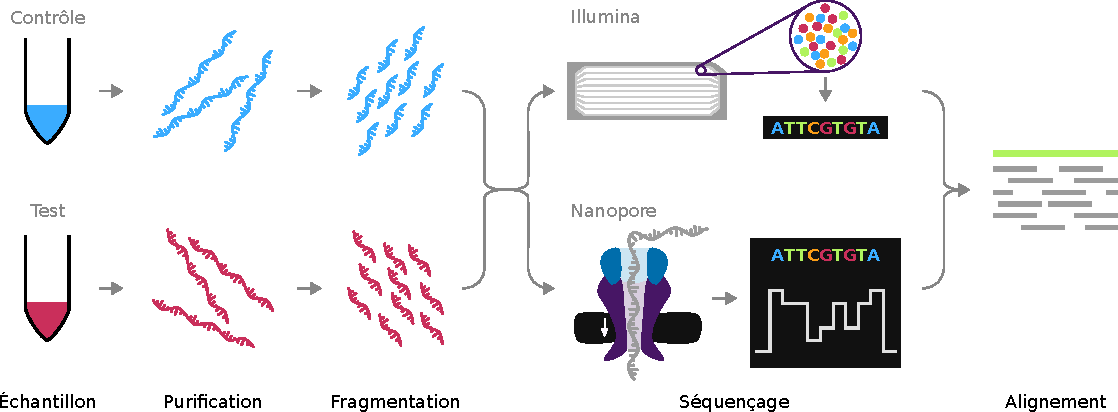
\includegraphics[width=\textwidth]{img/intro/2_meth_transcripto/intro_2_rnaseq_workflpow.pdf}
    \caption{Déroulé d'une opération de quantification d'expression par RNA-seq.}
    \label{fig:rnaseq_workflow}
\end{figure}


\subsubsection{Pré-traitement des données}

Le RNA-seq comme les puces à ADN nécessite de normaliser et transformer les données pour les rendre exploitable en retirant les biais techniques et biologiques. Des contrôles qualités existent ainsi pour contrôler dans un premier temps des artefacts de séquençage comme un k-mer sur-représenté, ou des erreurs de formatage ou encodage des fichiers par exemple. Du côté de la normalisation, si la division des comptes bruts par la profondeur de séquençage et 1 million qui donne des comptes par million (CPM et en anglais \textit{count per million}) est une normalisation consensus, d'autres normalisations couramment rencontrées ne peuvent être appliquées aussi systématiquement. La normalisation donnant des FPKM pour le séquençage à lecture par paire (en anglais \textit{paired-end}) ou RPKM lorsqu'il s'agit de séquençage à lecture unique (en anglais \textit{single end}) est ainsi une normalisation à éviter lors d'analyses comparatives \cite{Wagner2012Dec}. En divisant directement les CPM par la longueur des gènes pour tenir compte du biais de comptage en faveur des gènes de petite taille, les FPKM/RPKM entraînent potentiellement une somme de lectures normalisée différente dans chaque échantillon. L'analyse comparative étant un des intérêts majeur de la transcriptomique en recherche en médecine moléculaire et biologie, d'autres mesures normalisées compatibles ont été développées. Le RLE, pour \textit{Relative Log Expression} \cite{Anders2010Oct} et le TMM pour \textit{Trimmed Mean of M-values} \cite{Robinson2010Mar} sont ainsi des normalisations recommandées par l'étude du French StatOmique Consortium\footnote{Dans cette publication, le RLE est introduit par le biais du package DESeq \cite{Anders2010Oct} qui implémente cette mesure} en 2013 \cite{Dillies2013Nov}. Tous deux partent du principe que l'expression de la majorité des gènes ne change pas entre deux conditions. Le RLE consiste tout d'abord à calculer une pseudo référence (Équation \ref{pseudoref}) via une moyenne géométrique sur tous les échantillons \cite{Gandolfo2018Feb} qui contrairement au RPKM conserve bien une somme de lectures identique entre échantillons et est moins sensible aux valeurs extrêmes que la moyenne arithmétique. Un facteur de taille (Équation \ref{sizefactor} est ensuite calculé comme la médiane des rapports entre les comptages de chaque échantillon avec ceux de la pseudo-référence. Celui-ci est alors utilisé pour normaliser les comptes bruts de chaque échantillon.
% Celui-ci est alors utilisé pour calculer les paramètres $\mu_{i j}$ et $\sigma^2_{i j}$ de la loi binomiale négative qui sert à estimer les comptes de lectures d'un échantillon $j$ pour un gène $i$ (Équation \ref{readcount}).

\begin{equation}\label{pseudoref}
    \text{pseudo-référence} = \left(\prod_{t=1}^{m} k_{i t}\right)^{1 / m}
\end{equation}

\begin{equation}\label{sizefactor}
    \text{facteur de taille} = \hat{s}_{j}=\underset{i}{\operatorname{median}} \frac{k_{i j}}{\left(\prod_{v=t}^{m} k_{i t}\right)^{1 / m}}
\end{equation}

% \begin{equation}\label{readcount}
%     \text{comptes de lectures} = K_{i j} \sim NB(\mu_{i j}, \sigma^2_{i j})
% \end{equation}

Où :
\begin{align*}
i & = \text{gène} = 1,..., n \\
j & = \text{échantillon} = 1,..., m \\
k & = \text{table de comptes de lectures observés } n \times m 
\end{align*}

Le TMM quant à lui effectue une normalisation par le nombre de fragments d'ARN pour chaque gène dans chaque échantillon et s'en sert pour calculer la valeur M qui est rapport du niveau moyen en base 2, soit un log2 entre les échantillons de deux conditions (Équation \ref{mvalue}). Certains comptes pouvant être nulls ce que ne peut accepter un $log$, il est d'usage d'employer des pseudo-comptes qui sont des comptes auxquels on a ajouté 1 \cite{Booeshaghi2021Mar}. Parallèlement, il calcule la valeur A qui est la valeur absolue du niveau d'expression (Équation \ref{avalue}). Ces deux valeurs sont respectivement tronquées de 30\% et 5\% et servent à estimer une moyenne pondérée par référence (l'échantillon au quartile haut le plus proche de la moyenne des quartiles haut) (Équation \ref{weightedmean}) qui permet enfin de calculer le facteur de normalisation (Équation \ref{normtmmfactor}).

\begin{equation}\label{mvalue}
    M_g = \log_{2} \left(\frac{Y_{gk} / N_k}{Y_{gk'} / N_k'}\right)
\end{equation}

\begin{equation}\label{avalue}
    A_g = \frac{1}{2} \left(\log_{2} \left(\frac{Y_{gk}}{N_k} \right) + \log_2 \left(\frac{Y_{gk'}}{N_k'}\right)\right)
\end{equation}

\begin{equation}\label{weightedmean}
    w^r_{gk} = \frac{N_k - Y_{gk}}{N_k \times Y_{gk}} + \frac{N_r - Y_{gr}}{N_r \times Y_{gr}}
\end{equation}

\begin{equation}\label{normtmmfactor}
    \log_2{} (TMM^r_k) = \frac{\sum_{g \in G^*} w^r_{gk} \times M^r_{gk}}{\sum_{g \in G^*} w^r_{gk}}
\end{equation}

Où :
\begin{align*}
    g & = \text{gène} \\
    k & = \text{échantillon} \\
    N_{…} & = \text{nombre total de lectures pour … (soit }k \text{, soit r)} \\
    Y_{g…} & = \text{comptes observés pour … (soit }k \text{, soit r)} \\
    r & = \text{référence} \\
    G^* & = \text{ensemble des gènes non tronqués lors du tronquage de } M_g \text{ et } A_g
\end{align*}

% Now, double trim the upper and lower percentages of the data (trim M values by 30% and A values by 5%)
% Get weighted mean of M after trimming and calculate normalization factor 


Une étude détaillée des performances et propriétés mathématiques du RLE et du TMM a par ailleurs été publiée en 2016 en reprenant les différentes étapes de leur normalisation pour en tirer des équivalences \cite{Maza2016} (Figure \ref{fig:maza2016_table2}). On y mentionne d'ailleurs un filtÀ ces méthodes de normalisation s'ajoute des méthodes de normalisation se basant sur le contenu en GC qui va favoriser ou défavoriser le séquençage, ou encore des méthodes utilisant, à l'instar des puces à ADN, des gènes contrôle, le plus souvent des gènes dit de ménage (en anglais \textit{housekeeping genes}). Si elles peuvent être adaptées à certains contextes d'analyse, elles sont cependant peu ou pas utilisées dans ceux sur lesquels on se concentre par la suite dans cette thèse. 

\begin{figure}[!h]
    \centering
    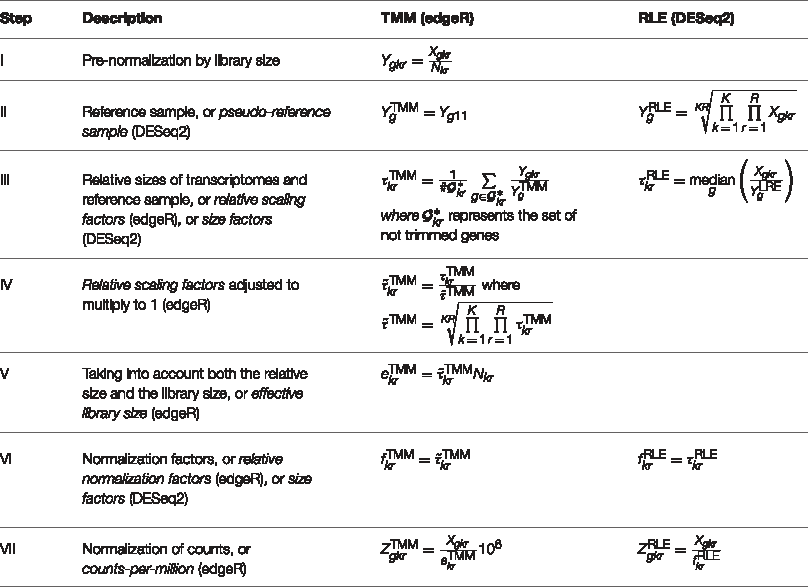
\includegraphics{img/intro/2_meth_transcripto/intro_2_maza2016_table2.pdf}
    \caption{Table de comparaison des étapes de normalisation avec équivalences re-exprimées. Issu de la Table 2 (tronquée) de Maza 2016 \cite{Maza2016}.}
    \label{fig:maza2016_table2}
\end{figure}






\section{L'analyse transcriptomique par réseaux de co-expression}

L'explosion de la taille et quantité de jeux de données mis à disposition publiquement engendre une demande croissante en techniques d'analyse capable de les gérer la masse et de profiter de la précision de séquençage apportée. 
% En recherche en médecine moléculaire et plus largement en biologie comparative, ce sont des méthodes d'étude des différences d'expression de gènes entre conditions qui ont été largement employées pour .
% Dépendant de la problématique à laquelle on cherche à répondre, il existe plusieurs méthodes. À l'aide de l'outil TopHat \cite{Trapnell2009May}, il est par exemple possible de faire de la découverte de variant à partir de données de RNA-seq pour expliquer des variations phénotypiques \cite{Bakhtiarizadeh2020Aug}. Toujours avec des données de RNA-seq, il est possible d'étudier les isoformes de transcrits pour un gène qui sont parfois responsables de pathologies \cite{Cooper2009Feb}.
% En réalisant
% Pour analyser des données de quantification d'expression, la méthode d'analyse d'expression différentielle fut très rapideemtn 
L'analyse d'expression différentielle fut la première méthode dédiée spécifiquement à l'analyse des données de quantification d'expression contrairement à des méthodes de statistique exploratoire comme l'analyse par composantes principales (ACP) \cite{deKok2005Jan}. Elle consiste à comparer l'expression de chaque gène entre des conditions, le plus souvent un contrôle contre un test, pour déterminer avec un test statistique quels gènes voient leur expression significativement changer dans la condition test. Si plusieurs méthodes ont été développées pour s'assurer de la robustesse d'identification \cite{Soneson2013Dec,Spies2019Jan}, le cœur de chacun reste le même : identifier les gènes sur-exprimés ou sous-exprimés. Dans la recherche permanente qu'est la priorisation de gènes candidats à une maladie, cette méthode a donc grandement contribué à la connaissance approfondie de certaines pathologies ainsi que permis d'y associer des biomarqueurs pour réaliser des diagnostics \cite{Costa-Silva2017Dec}. Outre les problèmes de reproductibilité soulevés par plusieurs études \cite{Ostlund2014}, les analyses d'expression différentielle présentent cependant l'inconvénient d'être limitées à quelques gènes d'un ou plusieurs mécanismes qui impliquent pourtant bien plus de gènes. À titre d'exemple, nombre de gènes associés à des maladies Mendéliennes sont exprimés dans plusieurs tissus sans entrainer nécessairement de disfonctionnement, suggérant  plus une interaction problématique \cite{Hekselman2020Mar}. De plus, l'analyse d'expression différentielle est mise en difficulté dans le cas de gènes à large variance étant donné la tendance à ces plages de variance à se chevaucher \cite{Ostlund2014}. Elle en vient alors à manquer des gènes dont l'implication est effective dans certaines conditions \cite{delaFuente2010Jul}. L'analyse par réseaux de co-expression de gènes s'est notamment développée dans l'optique de répondre à ce type de problématique. En ne considérant non pas seulement les gènes mais leur dynamique d'expression, leur synchronisation, les réseaux de co-expression visent à identifier les motifs de variation de la transcription qui indiquent des interactions fonctionnelles ou de régulation des relations entre gènes \cite{Parsana2019}.

% Barabási A-L, Gulbahce N, Loscalzo J. Network medicine: a network-based approach to human disease. Nat Rev Genet. 2011;12:56–68. + Furlong LI. Human diseases through the lens of network biology. Trends Genet. 2013;29:150–9.



\#\#\#\#\#\#\#\#\#\#\#\#\#\#\#\#\#\#\# FIN DE LA RÉDACTION PROPRE \#\#\#\#\#\#\#\#\#\#\#\#\#\#\#\#\#\#\#

% \subsection{Principe de la co-expression et définitions des réseaux}
\subsection{Définitions des réseaux et principe de la co-expression}

L'analyse par réseaux de co-expression de gènes (RCG, en anglais GCN pour \textit{Gene Co-expression Network}) a su bénéficier des avancées en théorie des réseaux depuis sa conception pour encoder au mieux les relations entre gènes et étudier les relations les liants \cite{Barabasi2011Jan}. La théorie des réseaux appartient elle-même à la théorie des graphes, structure mathématique derrière les réseaux \cite{Barnes1983Jun}. Ces derniers n'en sont en effet qu'une implémentation, un cas particulier pour représenter des entités et leur connections. Ainsi, si les termes de graphe et réseau sont souvent utilisés de façon interchangeable hors de la recherche en informatique et  mathématique, il est à noter qu'ils désignent des concepts différents bien qu'imbriqués, et au vocabulaire spécifique. Les entités considérées, ici les gènes, sont appelés "nœuds" dans un réseau et "sommets" dans un graphe. De même, les connections reliant les entités seront nommées respectivement "lien" et "arrête" et peuvent être porteuses d'une pondération représentant une valeur de la connexion. 


Les RCG se construisent conventionnellement à partir d'une matrice d'expression $n \times m$ d'indice $i = 1 … n$ pour les échantillons et de variable $j = 1 … m$ pour les gènes sur laquelle un score de similarité va être calculé. Ce terme généraliste permet d'englober la quantité importante de méthodes employée pour quantifier la similarité des gènes deux à deux. Ainsi, si ce score était initialement basé sur une approche naïve par corrélation de Pearson \cite{Carter2004}, d'autres scores plus robustes ont depuis été proposés. La corrélation de Spearman avec sa méthode est ainsi une méthode couramment utilisée en raison de sa sensibilité faible aux artefacts grâce à sa corrélation par rang \cite{Chowdhury2019,Serin2016,Kuehne2017}. Toujours dans les scores basés sur des coefficients de corrélation, la corrélation médiane bipondérée aussi appellée bicor \cite{Song2012} se base sur une corrélation par médiane qui se veut plus robuste que Pearson. Des mesures de distance sont aussi connues pour être utilisées en tant que score de similarité. C'est le cas de l'information mutuelle qui vise à mesurer la quantité d'information obtenable d'une variable en utilisant une autre pour estimer la dépendance entre celles-ci \cite{Kullback1997}. En définitive, le choix d'une de ces méthodes plus qu'une autre pour servir de score de similarité dépend de la nature des données (ex : linéaire ou non entre gènes) bien que la corrélation de Spearman et la bicor soient aujourd'hui les plus courantes \cite{Serin2016}.


En 1999, Barabasi découvrent une propriété de topologie à laquelle répondent la quasi totalité des réseaux de très grande taille comme les interactions entre gènes : l'invariance d'échelle (en anglais \textit{scale-free}).

% Continuer en parlant que ça a influé la theorie des reseaux et donc le developpement d'amelioration des scores de similarité en les transforamant en matrice d'adjacence. Plus tard Ritchie permettra à nouveau d'ameliorer ce score en amenant l'aspect de modularité topologique


\begin{figure}
    \centering
    % \includegraphics{}
    \caption{Étapes de réalisation d'une analyse par réseaux de co-expression.}
    \label{fig:coexpr_pipeline}
\end{figure}

% L'analyse par réseaux de co-expression se sépare généralement en 3 parties : la construction du réseau, la détection de groupes des gènes se co-exprimant et l'exploitation de ces derniers. 

Mélange historique / techniques
- approche naive : la correlation + méthode de clustering genre kmeans
- évolution vers l'utilisation de différentes métriques de distance et similarité


% Carter, "l'origine" 10.1093/bioinformatics/bth234

%% GROOOOOSSSE PUBLI REVIEW sur la co-expression ET la comparaison de modules, aka co-expr differentielle https://doi.org/10.1109/TCBB.2019.2893170

% https://www.mdpi.com/2073-4425/3/3/344/htm

% - Les types de réseaux/graphes rencontrés en biologie et plus particulièrement en expression des gènes : small-world


% ###### NORMALISAITON
% Normalization methods for RNA-seq data are different from those used for microarray data.
% Also for RNA-seq data there are several different methods that are being used, but not without
% debate. Fragments/Reads Per Kilobase of transcript per Million mapped reads (FPKM/RPKM)
% [61, 62] and Transcripts Per Million (TPM) [63] values, are normalization methods that correct
% for the total number of reads in a sample, as well as gene length [61]. One issue with these
% methods is that if a very highly expressed gene increases in expression, these normalization
% methods will make it appear as if all other genes decrease in expression. This is particularly
% important for co-expression analysis as it will create a false impression of positive co-
% expression between all these other genes
% These de Sipko van Damn

%% Relire `van Dam, S., Võsa, U., van der Graaf, A., Franke, L. & de Magalhães, J. P. Gene co-expression analysis for functional classification and gene–disease predictions. Brief. Bioinform. bbw139 (2017). doi:10.1093/bib/bbw139`
\begin{itemize}
    \item Réseaux binaires (0 = pas de connexion, 1 = connexion). Pour et contres.
    \item Réseaux pondérés. Pourquoi c'est vers ça qu'on s'est orientés ? Car les connections entre gènes ne sont pas binaires, elles sont plutot multiples et très dépendantes temporellement. Une meme cellule échantillonnée à des temps différents aura un profil plus ou moins différent. On y retrouvera les grandes fonctions clefs mais les aspects plus variables auront peut etre changé. D'où aussi la nécessité d'un bon nombre d'échantillons pour assurer la validité des résultats. Sinon les correlations ne sont pas représentatives.
\end{itemize}

\subsection{Construction}
\begin{itemize}
\item l'impact de l'utilisation de microarray ou plutôt de RNA-seq https://academic.oup.com/bioinformatics/article/29/6/717/184320
\item Pourquoi utiliser les counts plutôt que les FPKM, TPM, etc.
% In addition to the normalization issues that occur in single-cell RNA-seq, the optimal method for normalizing bulk RNA-seq data is also still not clear. The widely used Fragment/Reads Per Kilobase Million (FPKM) normalization has been debated [58] and although alternatives have and are being created, each method has its limitations (https://academic.oup.com/bib/article-lookup/doi/10.1093/bib/bbw139)
\item Quelles étapes de pré-traitement ?
\item Les différents scores de similarité : Pearson, Spearman, bicor, mutual information
\item La pondération des scores (adjacence et TOM) et la propriété d'invariance d'échelle (scale-free). Reparler de barbarasi et son celebre article (https://science.sciencemag.org/content/325/5939/412/tab-pdf) + Pourquoi elle est parfois encore discutée (https://www.nature.com/articles/s41467-019-08746-5) alors que tout de même pertinente en biologie. 
\end{itemize}
\subsection{Détection de modules}
\begin{itemize}
    \item Notion de communauté
    \item Définition du partitionnement (clustering) et des différentes techniques
\end{itemize}

\subsection{Exploitation des modules de gènes}

\subsubsection{Intégration biologique}
%% AKA knowledge driven
\begin{itemize}
    \item Enrichissement
    \item Test d'association
\end{itemize}

\subsubsection{Association phenotypique}
%% aussi knowledge driven

%%\subsection{Capitalisation sur l'information intrinsèque aux données}

\subsubsection{Étude topologique}
%% AKA data driven

%% Note : à voir si je présente aussi ici la comparaison de module vu que je vais ptet évoquer l'expression differentielle ici pour faire le parallele avec l'analyse transcripto classique. Sinon ça ira dans l'intro du chapitre avec l'article de GWENA.

\begin{itemize}
    \item Degré
    \item Définition de hub gene
    A trier / ordonner entre les différentes définitions, ce qu'elles visent, ce qu'elles appaortent et si possible une comparaison d'entre elles. On distinguera les mesure purement basées sur la theorie des graphs et celles impliquant des mesures statistique de significativité d'un gene comme hub (cf publi sur DHGA)
    \begin{itemize}
        \item Def 1 : Network theory : "A node is defined as hub node, if its connection degree is greater than average connection degree of the network" %% https://www.ncbi.nlm.nih.gov/pmc/articles/PMC5215982/
        \item Def 2 : Network hubs, the core elements in the network, can be defined using a range of different measures. These measures quantify distinct aspects of topological centrality, which can be defined as the capacity of a node to influence or be influenced by other nodes by virtue of its connection topology (Fornito et al., 2016).
    \end{itemize}
\end{itemize}
\subsubsection{Expression différentielle}
Pas sur de foutre ca là... Peut etre plutot en intro de la section complete en guise de "En analyse RNA classique, une méthode data driven est l'expression différentielle, mais en co-expression on a a disposition plus d'information extractable, et ce grace a la theorie des graphes" 

\subsubsection{Comparaison de modules}

Ou co-expression différentielle
%% "However, searching for differences in networks requires great sensitivity to the initial choice of data. For example, the absence of a shared link in mouse and human co-expression networks does not necessarily indicate divergent function. Instead, differences in the mouse and human co-expression networks may indicate differences in the technical platforms or the experimental conditions used to build the networks" http://doi.org/10.1371/journal.pgen.1000776

\subsection{Interprétation des résultats}

\subsubsection{Comparabilité des résultats issus de RNA-seq et de microarray}
\begin{itemize}
    \item Pas les meme hub genes %% "Microarray and RNA-seq-derived networks have different hub genes" https://academic.oup.com/bioinformatics/article/31/13/2123/196230
\end{itemize}


%%%%%%% L'INTÉRÊT DE l'ANALYSE PAR CO-EXPRESSION POUR L'ÉTUDE DU VIEILLISSEMENT %%%%%%%


\section{Le vieillissement, système hautement imbriqué}
%% Idée de début de paragraphe
S'il est une condition biologique où les réseaux de co-expression sont particulièrement bien adpatés, c'est bien le vieillissement. Source multi-factorielle de changements dans l'organisme, il est chez l'humain à l'origine d'une dégradation progressive des fonctions de base du corps.

% Aide à la justification de l'utilisation de la co-expression dans l'étude du vieillissement : 10.1016/j.arr.2009.10.006

%% GROSSE REVIEW : 10.1007/978-3-030-25650-0

\subsection{Définition biologique}

%% Liens utiles :
% The future of ageing https://www.nature.com/articles/35041709
% Bouquin vieillissement https://library.oapen.org/bitstream/handle/20.500.12657/24382/1005732.pdf?sequence=1#page=98
% Is mammalian aging genetically controlled https://sci-hub.se/https://link.springer.com/article/10.1023/A:1023356005749
% https://www.nature.com/articles/35041709
% https://www.nature.com/articles/nrm.2017.68 maladies définies comme associées à l'âge
% ACcumulation erreurs et lien avec la mortalité (page 123) https://www.sciencedirect.com/science/article/abs/pii/S095506741730131X
% Age dependant/independant mortality : https://en.wikipedia.org/wiki/Gompertz%E2%80%93Makeham_law_of_mortality
% REview biomarqueurs et forces d'action sur le vieillissement : https://sci-hub.se/10.1007/978-3-030-25650-0

% "Two evolutionary theories of ageing — the mutation-accumulation and trade-off theories "


%% À reformuler comme définition du vieillissement mais le contenu est sympa
% Aging is the inevitable time-dependent decline in physiological organ function and is a major risk factor for cancer development. Due to advances in health care, hygiene control and food availability, life expectancy is increasing and the population in most developed countries is shifting to an increasing proportion of people at a cancer susceptible age.

\begin{itemize}
    \item Phenomène à la fois génétique (intrinseque) [] et environemental (extrinseque) 
    \item Facteurs (hallmarks) : raccourcissement des télomères, phénomènes d'inflammation, réduction de la machinerie cellulaire
    % Sterile inflammation, also known as ‘inflammaging’, is a hallmark of ageing and a contributing factor to many age-related diseases ( https://doi.org/10.1093/gerona/glu057). 
    \item Manifestation : Ralentissement de la division cellulaire, développement de cellules non-fonctionnelles / nocives (aka tumeurs), malfonctionnement des tissus/organes
    \item Le vieillissement, contrairement aux maladies mendéliennes, est multifactoriel est se manifeste donc sous la forme d'un spectre
    \item Différence Âge chronologique / âge biologique
    \item Différence vieillissement (aging), longévité (longevity/lifespan), survie en bonne santé (health-span) 
\end{itemize}

\textbf{Bouts de textes récupérés de l'intro du chap2 car mieux ici}

Il se manifeste dans chacun sous des formes différentes avec pour certains
Une difficulté supplémentaire se présente alors lors de l'isolement de biomarqueurs : les changements biologiques entraînés par l'altération de ces biomarqueurs lors du vieillissement sont-ils 
entraînés par des mécanismes distincts au sain du tissu considéré ou bien sont-ils communs entre plusieurs changements et/ou tissus ?
% un phénomène local au tissu ou bien plus général avec une incidence dans le tissu considéré ?
% Sont-ils la cause ou la conséquence du vieillissement. 
Une même modification avec le temps telle que le raccourcissement des télomères (abordé en X.X.X\todo{ref intro vieillissement}) peut ainsi donner des affections variable selon le tissu : fibroses pulmonaires, des anémies aplasique, des dyskératoses congénitale, etc. \cite{Armanios2012} (Table \ref{table:tissu_telomere_effet}). 

\begin{table}[h]
\resizebox{\textwidth}{!}{
\begin{tabular}{m{0.2\textwidth}m{0.2\textwidth}m{0.6\textwidth}}
\textbf{Type de tissu}                                                                    & \textbf{Nom du tissu}                                            & \textbf{\begin{tabular}[c]{@{}l@{}}Manifestations pathologiques chez l'humain \\ avec syndromes télomériques\end{tabular}} \\ \hline
\multirow{4}{*}{\begin{tabular}[c]{@{}l@{}}Tissus à fort\\ renouvellement\end{tabular}}   & Peau                                                             & • Blanchissement prématuré des cheveux                                                                                     \\
                                                                                          & \begin{tabular}[c]{@{}l@{}}Moelle \\ osseuse\end{tabular}        & • Anémie aplastique                                                                                                        \\
                                                                                          & Immune                                                           & \begin{tabular}[c]{@{}l@{}}• Infections opportuniste\\ • Immunodéfiscience des cellules B, T et NK\end{tabular}            \\
                                                                                          & \begin{tabular}[c]{@{}l@{}}Épithélium \\ intestinal\end{tabular} & \begin{tabular}[c]{@{}l@{}}• Entérocolite\\ • Émoussement villositaire\end{tabular}                                        \\
\multirow{3}{*}{\begin{tabular}[c]{@{}l@{}}Tissus à faible\\ renouvellement\end{tabular}} & Poumon                                                           & \begin{tabular}[c]{@{}l@{}}• Emphysème prématuré\\ • Fibrose pulmonaire idiopathique\end{tabular}                          \\
                                                                                          & Foie                                                             & • Fibrose-cirrhose du foie cryptogénétique                                                                                 \\
                                                                                          & Os                                                               & \begin{tabular}[c]{@{}l@{}}• Ostéoporose\\ • Nécrose avasculaire\end{tabular}                                              \\
Cancer                                                                                    & Multi-tissus                                                     & \begin{tabular}[c]{@{}l@{}}• Cancers épithéliaux\\ • Hémopathies malignes\end{tabular}                                    
\end{tabular}
}
\caption[Phénotypes de maladies spécifiques aux organes si télomères courts]{Phénotypes de maladies spécifiques aux organes chez les humains ayant des télomères courts. Modifié d'après la Table 2 de Armanios 2012, \textit{The telomere syndromes} \cite{Armanios2012}}
\label{table:tissu_telomere_effet}
\end{table}



\subsection{Enjeux}

% Le vieillissement est un phénomène à distinguer de la longévité qui ne tient pas compte de l'aspect dégradation de la santé. 

% Inflammaging and Garb-aging : https://www.sciencedirect.com/science/article/abs/pii/S1043276016301254
% Epigenetic, inflammationa and aging : https://www.sciencedirect.com/science/article/pii/B9780123978035000083

% Si la quête pour l'immortalité n'est pas souhaitable pour plusieurs raisons tant éthiques qu'économiques \cite{Hayflick2000}, la recherche pour un vieillissement en bonne santé se doit-elle de continuer.

De Magalhães s'interrogeait en 2003 \cite{deMagalhes2003} d'une programmation génétique du vieillissement. La question sous-jacente abordée était finalement de savoir si analyser et comprendre indépendemment chaque conséquence néfaste et maladie apparaissant avec l'âge n'était pas une course perdue d'avance pour les combattre. Ainsi, De Magalhães envisageait que comprendre le fonctionnement global du vieillissement serait plus pérenne pour retarder d'un seul coup l'apparition de quelques, si ce n'est toutes, maladies chez la personne âgée.

Le vieillissement est donc, part les pathologies qu'il entraîne, un enjeu de santé publique.


\begin{itemize}
    \item Susceptibilité aux maladies opportunistes
    \item tdeetAutonomie patient
    \item Médicalisation précoce
\end{itemize}

\subsection{La capture de l'information liée au vieillissement par la transcriptomique}
\label{}

\begin{itemize}
    \item La dérégulation de la transcription comme phénomène précédemment mentionné
    \item L'analyse d'expression différentielle + d'autres analyses discrètes (au sens de Barabasi) ont permis d'isoler plusieurs gènes associés à un ou plusieurs tissu vieillissant. \label{intro_biomarker_aging}
    \item la création de bases de données liées au vieillissement sous toutes ses formes : gènes associés au vieillissement dans différents tissus et chez différentes espèces modèle, signatures de scenescence, gènes associés au ralentissement du vieillissement par restriction calorique, médicaments anti vieillissement, gènes associés à la longévité, changements liés au vieillissement à différents niveaux (biological levels, integrating molecular, physiological and pathological age-relate). En gros tout https://genomics.senescence.info/
    \item L'insuffisance de la capture de biomarqueurs pour un processus aussi compliqué que le vieillissement. Donc la nécessité d'une étude en réseau
    \item 
    
\end{itemize}
%% https://doi.org/10.1007/978-981-32-9005-1_3
%% https://www.sciencedirect.com/science/article/abs/pii/S0959438820300878
%% https://onlinelibrary.wiley.com/doi/abs/10.1111/acel.13280

\section*{Phrases utiles à retravailler et intégrer}

\begin{itemize}
\item "Studies have shown that each gene is estimated on average to interact with four to eight other genes1 and to be involved in 10 biological functions" [10.1038/s41598-017-18705-z]
\item "A very clear partition of different biological networks is provided by Christensen et al. [1], who separated these networks into five main categories as follows: [metabolic networks, signal transduction networks,transcriptional regulatory networks, protein-protein networks, functional gene networks]" [10.1093/bfgp/elt003]
%% Bouquin à la coloc de Clément à Sète, pas retrouvé sur le net jusque là 
\item "Le vieillissement est un continuum conduisant une personne en bonne santé à une réduction de sa réserve fonctionnelle, puis de sa capacité fonctionnelle et de sa qualité de vie. CEs différents aspects ne décrivent pas un chemin linéaire ou ordonné." [Patient agé : particularités de la consultation, Gilles Berrut]
\item "It has been reported that nearly one in four studies uses public data to address a biological problem without generating new raw data (Rung and Brazma, 2013)." [10.3389/fpls.2016.00444]
\end{itemize}


%% Points que je veux aborder :
%%  - Definition des reseau arrete / noeud
%%  - Definition des modules par l'effet de modularité
%%  - Ce à quoi ils peuvent servir : raccrochage de fonction a certains genes, detection de pathways, detection de reseaux de regulation



%%    • Weighted aspect [trop general, aura plutot sa place dans la thèse]
%% But because of the multi-functionality aspect of each gene, such GCN using only binary state between genes (1 = correlated, 0 = not correlated) lead to information loss\cite{Langfelder2008}. Therefore, a new class of GCN have been developed: weighted gene co-expression networks. One of the most famous implementation is the R package WGCNA\cite{Langfelder2008}, but one can also mention the recent wTO\cite{Gysi2018} package which consider both positive and negative correlation for GCN building. Instead of a simple pairwise correlation, these packages weight the similarity score by calculating a factor taking into account other properties of the network. In the case of WGCNA, it specifies an adjacency score which raise the similarity to a power, which will increase the strength of strong similarities while keeping low week ones. In the case of wTO, it determine an average accounting for all common neighbors of a node.

%%    • Topological aspect
%%    • Co-expression properties (Scale-free-network entre autres ?)



%% Infos sur la peau : these super interessante => https://dumas.ccsd.cnrs.fr/dumas-01599807/document% \end{itemize}

% ###########################################################################################################

\section{Motivations et hypothèses de recherche}

%% Reprendre la fin d'intro/intro pour guider

